%%%%%%%%%%%%%%%%%%%%%%%%%%%%%%%%%%%%%%%%%%%%%%%%%%%%%%%%%%%%%%%%%%%%%%%%%
%  Zawartość: Główny plik szablonu pracy dyplomowej (magisterskiej/inżynierskiej).
%  Opracował: Tomasz Kubik <tomasz.kubik@pwr.edu.pl>
%  Data: kwiecień 2016
%  Wersja: 0.2
%%%%%%%%%%%%%%%%%%%%%%%%%%%%%%%%%%%%%%%%%%%%%%%%%%%%%%%%%%%%%%%%%%%%%%%%%

\documentclass[a4paper,onecolumn,oneside,12pt,extrafontsizes]{memoir}
% W celu przygotowania wydruku do archiwum należy przesłonić komendę powyższą
% dwoma poniższymi komendami:
%\documentclass[a4paper,onecolumn,twoside,10pt]{memoir} 
%\renewcommand{\normalsize}{\fontsize{8pt}{10pt}\selectfont}

%\usepackage[cp1250]{inputenc} % jeśli kodowanie edytowanych plików to cp1250 
\usepackage[utf8]{inputenc} % jeśli kodowanie edytowanych plików to UTF8
\usepackage[T1]{fontenc}
\usepackage[english]{babel}
%\DisemulatePackage{setspace}
\usepackage{setspace}
\usepackage{tabularx}
\usepackage{color,calc}
%\usepackage{soul} % pakiet z komendami do podkreślania tekstu

\usepackage{ebgaramond} % pakiet z czcionkami garamond, potrzebny tylko do strony tytułowej, musi wystąpić przed pakietem tgtermes

%% Aby uzyskać polskie literki w pdfie (a nie zlepki) korzystamy z pakietu czcionek tgterms. 
%% W pakiecie tym są zdefiniowane klony czcionek Times o kształtach: normalny, pogrubiony, italic, italic pogrubiony.
%% W pakiecie tym brakuje czcionki o kształcie: slanted (podobny do italic). 
%% Jeśli w dokumencie gdzieś zostanie zastosowana czcionka slanted (np. po użyciu komendy \textsl{}), to
%% latex dokona podstawienia na czcionkę standardową i zgłosi to w ostrzeżeniu (warningu).
%% Ponadto tgtermes to czcionka do tekstu. Wszelkie matematyczne wzory będą sformatowane domyślną czcionką do wzorów.
%% Jeśli wzory mają być sformatowane z wykorzystaniem innych czcionek, trzeba to jawnie zadeklarować.

%% Po zainstalowaniu pakietu tgtermes może będzie trzeba zauktualizować informacje 
%% o dostępnych fontach oraz mapy. Można to zrobić z konsoli (jako administrator)
%% initexmf --admin --update-fndb
%% initexmf --admin --mkmaps

\usepackage{tgtermes}   
\renewcommand*\ttdefault{txtt}

% We wcześniejszej wersji szablonu korzystano z innych czcionek. Dla celów historycznych pozostawiono je w komentarzu
%\usepackage{mathptmx} % pakiet będący następcą pakietów times and mathptm, niestety polskie literki są zlepkami
%\usepackage{newtxtext,newtxmath} % pakiety dostarczające Times dla tekstów i wzorów matematycznych,  
%                                  rozwiązuje problemy występujące w mathptmx, ale wymaga zainstalowania
%                                  dodatkowych pakietów oraz uruchomienia updmap (konsola administratora)
%                                  niestety polskie literki są zlepkami
%\usepackage{newtxmath,tgtermes} % można też połączyć czcionki do tekstu i czcionki do wzorów

\usepackage{listings} % pakiet do prezentacji kodu. 
%Wcześniej był problem z polskimi znakami w otoczeniu lstlisting, stąd pozostawiono w komentarzu zastosowane wtedy rozwiązanie: 
\lstset{literate=%-
{ą}{{\k{a}}}1 {ć}{{\'c}}1 {ę}{{\k{e}}}1 {ł}{{\l{}}}1 {ń}{{\'n}}1 {ó}{{\'o}}1 {ś}{{\'s}}1 {ż}{{\.z}}1 {ź}{{\'z}}1 {Ą}{{\k{A}}}1 {Ć}{{\'C}}1 {Ę}{{\k{E}}}1 {Ł}{{\L{}}}1 {Ń}{{\'N}}1 {Ó}{{\'O}}1 {Ś}{{\'S}}1 {Ż}{{\.Z}}1 {Ź}{{\'Z}}1 }%{\ \ }{{\ }}1}

% Choć możliwe jest zastosowanie różnych pakietów formatujących tabele, zaleca się tego nie robić.
%\usepackage{longtable}
%\usepackage{ltxtable}
%\usepackage{tabulary}

%%%%%%%%%%%%%%%%%%%%%%%%%%%%%%%%%%%%%%%%%%%%%%%%%%%
%% Ustawienia odpowiedzialne za sposób łamania dokumentu
%% i ułożenie elementów pływających
%%%%%%%%%%%%%%%%%%%%%%%%%%%%%%%%%%%%%%%%%%%%%%%%%%%
%\hyphenpenalty=10000		% nie dziel wyrazów zbyt często
\clubpenalty=10000      %kara za sierotki
\widowpenalty=10000  % nie pozostawiaj wdów
\brokenpenalty=10000		% nie dziel wyrazów między stronami
\exhyphenpenalty=999999		% nie dziel słów z myślnikiem
\righthyphenmin=3			% dziel minimum 3 litery

%\tolerance=4500
%\pretolerance=250
%\hfuzz=1.5pt
%\hbadness=1450

\renewcommand{\topfraction}{0.95}
\renewcommand{\bottomfraction}{0.95}
\renewcommand{\textfraction}{0.05}
\renewcommand{\floatpagefraction}{0.35}

%%%%%%%%%%%%%%%%%%%%%%%%%%%%%%%%%%%%%%%%%%%%%%%%%%%
%%  Ustawienia rozmiarów: tekstu, nagłówka i stopki, marginesów
%%  dla dokumentów klasy memoir 
%%%%%%%%%%%%%%%%%%%%%%%%%%%%%%%%%%%%%%%%%%%%%%%%%%%
\setlength{\headsep}{10pt} 
\setlength{\headheight}{13.6pt} % wartość baselineskip dla czcionki 11pt tj. \small wynosi 13.6pt
\setlength{\footskip}{\headsep+\headheight}
\setlength{\uppermargin}{\headheight+\headsep+1cm}
\setlength{\textheight}{\paperheight-\uppermargin-\footskip-1.5cm}
\setlength{\textwidth}{\paperwidth-5cm}
\setlength{\spinemargin}{2.5cm}
\setlength{\foremargin}{2.5cm}
\setlength{\marginparsep}{2mm}
\setlength{\marginparwidth}{2.3mm}
%\settrimmedsize{297mm}{210mm}{*}
%\settrims{0mm}{0mm}	
\checkandfixthelayout[fixed] % konieczne, aby się dobrze wszystko poustawiało
%%%%%%%%%%%%%%%%%%%%%%%%%%%%%%%%%%%%%%%%%%%%%%%%
%%  Ustawienia odległości linii, wcięć, odstępów
%%%%%%%%%%%%%%%%%%%%%%%%%%%%%%%%%%%%%%%%%%%%%%%%
\linespread{1}
%\linespread{1.241}
\setlength{\parindent}{14.5pt}
%\setbeforesecskip{10pt plus 0.5ex}%{-3.5ex \@plus -1ex \@minus -.2ex}
%\setaftersecskip{10pt plus 0.5ex}%\onelineskip}
%\setbeforesubsecskip{8pt plus 0.5ex}%{-3.5ex \@plus -1ex \@minus -.2ex}
%\setaftersubsecskip{8pt plus 0.5ex}%\onelineskip}
%\setlength\floatsep{6pt plus 2pt minus 2pt} 
%\setlength\intextsep{12pt plus 2pt minus 2pt} 
%\setlength\textfloatsep{12pt plus 2pt minus 2pt} 

%%%%%%%%%%%%%%%%%%%%%%%%%%%%%%%%%%%%%%%%%%%%%%%%%%%
%%  Pakiety i komendy zastosowane tylko do zamieszczenia informacji o użytych komendach i fontach
%%  Normalnie nie są potrzebne, można je zamarkować podczas redakcji pracy
%%%%%%%%%%%%%%%%%%%%%%%%%%%%%%%%%%%%%%%%%%%%%%%%%%%
\usepackage{memlays}     % extra layout diagrams, zastosowane w szblonie do 'debuggowania', używa pakietu layouts
%\usepackage{layouts}
\usepackage{printlen} % pakiet do wyświetlania wartości zdefiniowanych długości, stosowany do 'debuggowania'
\uselengthunit{pt}
\makeatletter
\newcommand{\showFontSize}{\f@size pt} % makro wypisujące wielkość bieżącej czcionki
\makeatother
% do pokazania ramek można byłoby użyć:
%\usepackage{showframe} 


%%%%%%%%%%%%%%%%%%%%%%%%%%%%%%%%%%%%%%%%%%%%%%%%%%%
%%  Formatowanie list wyliczeniowych, wypunktowań i własnych otoczeń
%%%%%%%%%%%%%%%%%%%%%%%%%%%%%%%%%%%%%%%%%%%%%%%%%%%

% Domyślnie wypunktowania mają zadeklatorowane znaki, które nie występują w tgtermes
% Aby latex nie podstawiał w ich miejsca znaków z czcionki standardowej można zrobić podstawienie:
%    \DeclareTextCommandDefault{\textbullet}{\ensuremath{\bullet}}
%    \DeclareTextCommandDefault{\textasteriskcentered}{\ensuremath{\ast}}
%    \DeclareTextCommandDefault{\textperiodcentered}{\ensuremath{\cdot}}
% Jednak jeszcze lepszym pomysłem jest zdefiniowanie otoczeń z wykorzystaniem enumitem
\usepackage{enumitem} % pakiet pozwalający zarządzać formatowaniem list wyliczeniowych
\setlist{noitemsep,topsep=4pt,parsep=0pt,partopsep=4pt,leftmargin=*} % zadeklarowane parametry pozwalają uzyskać 'zwartą' postać wypunktowania bądź wyliczenia
\setenumerate{labelindent=0pt,itemindent=0pt,leftmargin=!,label=\arabic*.} % można zmienić \arabic na \alph, jeśli wyliczenia mają być z literkami
\setlistdepth{4} % definiujemy głębokość zagnieżdżenia list wyliczeniowych do 4 poziomów
\setlist[itemize,1]{label=$\bullet$}  % definiujemy, jaki symbol ma być użyty w wyliczeniu na danym poziomie
\setlist[itemize,2]{label=\normalfont\bfseries\textendash}
\setlist[itemize,3]{label=$\ast$}
\setlist[itemize,4]{label=$\cdot$}
\renewlist{itemize}{itemize}{4}

%%%http://tex.stackexchange.com/questions/29322/how-to-make-enumerate-items-align-at-left-margin
%\renewenvironment{enumerate}
%{
%\begin{list}{\arabic{enumi}.}
%{
%\usecounter{enumi}
%%\setlength{\itemindent}{0pt}
%%\setlength{\leftmargin}{1.8em}%{2zw} % 
%%\setlength{\rightmargin}{0zw} %
%%\setlength{\labelsep}{1zw} %
%%\setlength{\labelwidth}{3zw} % 
%\setlength{\topsep}{6pt}%
%\setlength{\partopsep}{0pt}%
%\setlength{\parskip}{0pt}%
%\setlength{\parsep}{0em} % 
%\setlength{\itemsep}{0em} % 
%%\setlength{\listparindent}{1zw} % 
%}
%}{
%\end{list}
%}

\makeatletter
\renewenvironment{quote}{
	\begin{list}{}
	{
	\setlength{\leftmargin}{1em}
	\setlength{\topsep}{0pt}%
	\setlength{\partopsep}{0pt}%
	\setlength{\parskip}{0pt}%
	\setlength{\parsep}{0pt}%
	\setlength{\itemsep}{0pt}
	}
	}{
	\end{list}}
\makeatother

%%%%%%%%%%%%%%%%%%%%%%%%%%%%%%%%%%%%%%%%%
%%  Pakiet do generowania indeksu (ważne, aby wstawić przed hyperref)
%%%%%%%%%%%%%%%%%%%%%%%%%%%%%%%%%%%%%%%%%
\DisemulatePackage{imakeidx}
\usepackage[makeindex,noautomatic]{imakeidx} % tutaj mówimy, żeby indeks nie generował się automatycznie, 

%\usepackage[noautomatic]{imakeidx} 
\makeindex

\makeatletter
%%%\renewenvironment{theindex}
							 %%%{\vskip 10pt\@makeschapterhead{\indexname}\vskip -3pt%
								%%%\@mkboth{\MakeUppercase\indexname}%
												%%%{\MakeUppercase\indexname}%
								%%%\vspace{-3.2mm}\parindent\z@%
								%%%\renewcommand\subitem{\par\hangindent 16\p@ \hspace*{0\p@}}%%
								%%%\phantomsection%
								%%%\begin{multicols}{2}
								%%%%\thispagestyle{plain}
								%%%\parindent\z@                
								%%%%\parskip\z@ \@plus .3\p@\relax
								%%%\let\item\@idxitem}
							 %%%{\end{multicols}\clearpage}
%%%
\makeatother


\usepackage{ifpdf}
%\newif\ifpdf \ifx\pdfoutput\undefined
%\pdffalse % we are not running PDFLaTeX
%\else
%\pdfoutput=1 % we are running PDFLaTeX
%\pdftrue \fi
\ifpdf
 \usepackage[pdftex,bookmarks,breaklinks,unicode]{hyperref}
 \usepackage[pdftex]{graphicx}
 \DeclareGraphicsExtensions{.pdf,.jpg,.mps,.png}
\pdfcompresslevel=9
\pdfoutput=1
\makeatletter
\AtBeginDocument{
  \hypersetup{
	pdfinfo={
    Title = {\@title},
    Author = {\@author},
    Subject={},
    Keywords={słowa kluczowe},
  }}
}
\makeatother
\else
\usepackage{graphicx}
\DeclareGraphicsExtensions{.eps,.ps,.jpg,.mps,.png}
\fi
\sloppy


%\graphicspath{{rys01/}{rys02/}}


%%%%%%%%%%%%%%%%%%%%%%%%%%%%%%%%%%%%%%%%%
% Metadane dla pdfa


%\ifpdf
%\pdfinfo{
   %/Author (Nicola Talbot)
   %/Title  (Creating a PDF document using PDFLaTeX)
   %/CreationDate (D:20040502195600)
   %/ModDate (D:\pdfdate)
   %/Subject (PDFLaTeX)
   %/Keywords (PDF;LaTeX)
%}
%\fi

% Deklaracja głębokościu numeracji
\setcounter{secnumdepth}{2}
\setcounter{tocdepth}{2}
\setsecnumdepth{subsection} % activating subsubsec numbering in doc


% Kropki po numerach sekcji
\makeatletter
\def\@seccntformat#1{\csname the#1\endcsname.\quad}
\def\numberline#1{\hb@xt@\@tempdima{#1\if&#1&\else.\fi\hfil}}
\makeatother

\renewcommand{\chapternumberline}[1]{#1.\quad}
\renewcommand{\cftchapterdotsep}{\cftdotsep}

%\definecolor{niceblue}{rgb}{.168,.234,.671}

% Czcionka do podpisów tabel i rysunków
\captionnamefont{\small}
\captiontitlefont{\small}
% makro pozwalające zmienić sposób wypisywania rozdziału
%\def\printchaptertitle##1{\fonttitle \space \thechapter.\space ##1} 

%\usepackage{ltcaption}
% The ltcaption package supports \CaptionLabelFont & \CaptionTextFont introduced by the NTG document classes
%\renewcommand\CaptionLabelFont{\small}
%\renewcommand\CaptionTextFont{\small}

% Przedefiniowanie etykiet w podpisach tabel i rysunków
%\AtBeginDocument{% 
        \addto\captionspolish{% 
        \renewcommand{\tablename}{Tab.}% 
}%} 

%\AtBeginDocument{% 
%        \addto\captionspolish{% 
%        \renewcommand{\chaptername}{Rozdział}% 
%}} 

%\AtBeginDocument{% 
        \addto\captionspolish{% 
        \renewcommand{\figurename}{Rys.}% 
}%}


%\AtBeginDocument{% 
        \addto\captionspolish{% 
        \renewcommand{\bibname}{Literatura}% 
}%}

%\AtBeginDocument{% 
        \addto\captionspolish{% 
        \renewcommand{\listfigurename}{Spis rysunków}% 
}%}

%\AtBeginDocument{% 
        \addto\captionspolish{% 
        \renewcommand{\listtablename}{Spis tabel}% 
}%}

%\AtBeginDocument{% 
        \addto\captionspolish

%%%%%%%%%%%%%%%%%%%%%%%%%%%%%%%%%%%%%%%%%%%%%%%%%%%%%%%%%%%%%%%%%%                  
%% Definicje stopek i nagłówków
%%%%%%%%%%%%%%%%%%%%%%%%%%%%%%%%%%%%%%%%%%%%%%%%%%%%%%%%%%%%%%%%%%                  
\addtopsmarks{headings}{%
\nouppercaseheads % added at the beginning
}{%
\createmark{chapter}{both}{shownumber}{}{. \space}
%\createmark{chapter}{left}{shownumber}{}{. \space}
\createmark{section}{right}{shownumber}{}{. \space}
}%use the new settings

\makeatletter
\copypagestyle{outer}{headings}
\makeoddhead{outer}{}{}{\small\itshape\rightmark}
\makeevenhead{outer}{\small\itshape\leftmark}{}{}
\makeoddfoot{outer}{\small\@author:~\@titleShort}{}{\small\thepage}
\makeevenfoot{outer}{\small\thepage}{}{\small\@author:~\@title}
\makeheadrule{outer}{\linewidth}{\normalrulethickness}
\makefootrule{outer}{\linewidth}{\normalrulethickness}{2pt}
\makeatother

% fix plain
\copypagestyle{plain}{headings} % overwrite plain with outer
\makeoddhead{plain}{}{}{} % remove right header
\makeevenhead{plain}{}{}{} % remove left header
\makeevenfoot{plain}{}{}{}
\makeoddfoot{plain}{}{}{}

\copypagestyle{empty}{headings} % overwrite plain with outer
\makeoddhead{empty}{}{}{} % remove right header
\makeevenhead{empty}{}{}{} % remove left header
\makeevenfoot{empty}{}{}{}
\makeoddfoot{empty}{}{}{}


%%%%%%%%%%%%%%%%%%%%%%%%%%%%%%%%%%%%%%%
%% Definicja strony tytułowej 
%%%%%%%%%%%%%%%%%%%%%%%%%%%%%%%%%%%%%%%
\makeatletter
%Uczelnia
\newcommand\uczelnia[1]{\renewcommand\@uczelnia{#1}}
\newcommand\@uczelnia{}
%Wydział
\newcommand\wydzial[1]{\renewcommand\@wydzial{#1}}
\newcommand\@wydzial{}
%Kierunek
\newcommand\kierunek[1]{\renewcommand\@kierunek{#1}}
\newcommand\@kierunek{}
%Specjalność
\newcommand\specjalnosc[1]{\renewcommand\@specjalnosc{#1}}
\newcommand\@specjalnosc{}
%Tytuł po angielsku
\newcommand\titleEN[1]{\renewcommand\@titleEN{#1}}
\newcommand\@titleEN{}
%Tytuł krótki
\newcommand\titleShort[1]{\renewcommand\@titleShort{#1}}
\newcommand\@titleShort{}
%Promotor
\newcommand\promotor[1]{\renewcommand\@promotor{#1}}
\newcommand\@promotor{}

%\usepackage[absolute]{textpos} % zamarkowano, bo ostatecznie wykorzystano otoczenie picture

\def\maketitle{%
  \pagestyle{empty}%
%%\garamond 
	\fontfamily{\ebgaramond@family}\selectfont % na stronie tytułowej czcionka garamond
%%%%%%%%%%%%%%%%%%%%%%%%%%%%%%%%%%%%%	
%% Poniżej, w otoczniu picture, wstawiono tytuł i autora. 
%% Tytuł (z autorem) musi znaleźć się w obszarze 
%% odpowiadającym okienku 110mmx75mm, którego lewy górny róg 
%% jest w położeniu 77mm od lewej i 111mm od górnej  krawędzi strony 
%% (tak wynika z wycięcia na okładce). 
%% Poniższy kod musi być użyty dokładnie w miejscu gdzie jest.
%% Jeśli tytuł nie mieści się w okienku, to należy tak pozmieniać 
%% parametry użytych komend, aby ten przydługi tytuł jednak 
%% upakować go do okienka.
%%
%% Sama okładka (kolorowa strona z wycięciem, do pobrania z dydaktyki) 
%% powinna być przycięta o 3mm od każdej z krawędzi.
%% Te 3mm pewnie zostawiono na ewentualne spady czy też specjalną oprawę.
%%%%%%%%%%%%%%%%%%%%%%%%%%%%%%%%%%%%%	
\newlength{\tmpfboxrule}
\setlength{\tmpfboxrule}{\fboxrule}
\setlength{\fboxsep}{2mm}
\setlength{\fboxrule}{0mm} 
%\setlength{\fboxrule}{0.1mm} %% jeśli chcemy zobaczyć ramkę
\setlength{\unitlength}{1mm}
\begin{picture}(0,0)
\put(26,-124){\fbox{
\parbox[c][71mm][c]{104mm}{\centering%\lineskip=34pt 
\fontsize{16pt}{18pt}\selectfont \@titleEN\\[5mm]
\fontsize{16pt}{18pt}\selectfont \@title\\[20mm]
\fontsize{16pt}{18pt}\selectfont AUTHOR:\\[2mm]
\fontsize{14pt}{16pt}\selectfont \@author}
}
}
\end{picture}
\setlength{\fboxrule}{\tmpfboxrule} 
%%%%%%%%%%%%%%%%%%%%%%%%%%%%%%%%%%%%%
%% Reszta strony z nazwą uczelni, wydziału, kierunkiem, specjalnością
%% promotorem, oceną pracy, miastem i rokiem
	{\centering%\vspace{-1cm}
		{\fontsize{22pt}{24pt}\selectfont \@uczelnia}\\[0.4cm]
		{\fontsize{22pt}{24pt}\selectfont \@wydzial}\\[0.5cm]
		  \hrule %\vspace*{0.7cm}
	}
{\flushleft\fontsize{14pt}{16pt}\selectfont%
\begin{tabular}{ll}
FIELD: & \@kierunek\\
SPECIALIZATION: & \@specjalnosc\\
\end{tabular}\\[1.3cm]
}
{\centering
{\fontsize{32pt}{36pt}\selectfont ENGINEERING}\\[0.5cm]
{\fontsize{32pt}{36pt}\selectfont THESIS}\\[2.5cm]
}
\vfill
\begin{tabularx}{\linewidth}{p{6cm}l}
		&{\fontsize{16pt}{18pt}\selectfont SUPERVISOR:}\\[2mm] %UWAGA: tutaj jest miejsce na nazwisko promotora pracy
		&{\fontsize{14pt}{16pt}\selectfont \@promotor}\\[10mm]
		&{\fontsize{16pt}{18pt}\selectfont GRADE:}\\[20mm]
	\end{tabularx}
\vspace{2cm}
\hrule\vspace*{0.3cm}
{\centering
{\fontsize{16pt}{18pt}\selectfont \@date}\\[0cm]
}
%\ungaramond
\normalfont
 \cleardoublepage
}
\makeatother
%%%%%%%%%%%%%%%%%%%%%%%%%%%%%%%%%%%%%%%%%

%\AtBeginDocument{\addtocontents{toc}{\protect\thispagestyle{empty}}}




%%%%%%%%%%%%%%%%%%%%%%%%%%%%%%%%%%%%%%%%%
%%  Metadane dokumentu 
%%%%%%%%%%%%%%%%%%%%%%%%%%%%%%%%%%%%%%%%%
\title{Aplikacja mobilna zapewniająca dostęp offline do danych publikowanych w systemie obsługi studentów}
\titleShort{Mobile application providing offline access...}
\titleEN{Mobile application providing offline access to data published in a student services system}
\author{Justyna Skalska}
\uczelnia{WROCŁAW UNIVERSITY OF SCIENCE AND TECHNOLOGY}
\wydzial{FACULTY OF ELECTRONICS}
\kierunek{INFORMATYKA}
\specjalnosc{INŻYNIERIA SYSTEMÓW INFORMATYCZNYCH}
\promotor{Dr inż Tomasz Kubik, K-9}
\date{WROCŁAW, 2020}

% Ustawienie odstępu od góry w nienumerowanych rozdziałach oraz wykazach:
% Spis treści, Spis tabel, Spis rysunków, Indeks rzeczowy

%\newlength{\linespace}
%\setlength{\linespace}{-\beforechapskip-\topskip+\headheight+\topsep}
%\makechapterstyle{noNumbered}{%
%\renewcommand\chapterheadstart{\vspace*{\linespace}}
%}

%% powyższa komenda załatwia to, co robią komendy poniższe dla spisów
%\renewcommand*{\tocheadstart}{\vspace*{\linespace}}
%\renewcommand*{\lotheadstart}{\vspace*{\linespace}}
%\renewcommand*{\lofheadstart}{\vspace*{\linespace}}

%%%%%%%%%%%%%%%%%%%%%%%%%%%%%%%%%%%%%%%%%
%                  Początek dokumentu 
%%%%%%%%%%%%%%%%%%%%%%%%%%%%%%%%%%%%%%%%%
%\includeonly{skroty,rozdzial01} % jeśli chcemy kompilować tylko fragmenty, to można tu je wpisać

\begin{document}
% Tutaj można przełączyć odstęp między liniami
%\SingleSpacing
%\OnehalfSpacing
%\DoubleSpacing

%\settypeoutlayoutunit{cm} % do debugowania
%\typeoutstandardlayout    % wypisuje na stdout informacje o ustawieniach
\maketitle
\newpage


\chapterstyle{noNumbered}
\pagestyle{outer}
\mbox{}\pdfbookmark[0]{Spis treści}{spisTresci.1}
\tableofcontents* 

\newpage
\mbox{}\pdfbookmark[0]{Spis rysunków}{spisRysunkow.1}
%\addcontentsline{toc}{chapter}{Spis rysunków}
\listoffigures*
\begin{flushleft}

\end{flushleft}
%{%
%\let\oldnumberline\numberline%
%\renewcommand{\numberline}{\figurename~\oldnumberline}%
%\listoffigures%
%}


\newpage
\mbox{}\pdfbookmark[0]{Spis tabel}{spisTabel.1}
%\addcontentsline{toc}{chapter}{Spis tabel}
\listoftables*

\chapter*{Abbreviations}\mbox{}\pdfbookmark[0]{Skróty}{skroty.1}
\label{sec:skroty}
\noindent
\begin{description}
  \item [JIT] (\emph{Just-In-Time})
  \item [AOT] (\emph{Ahead-Of-Time})
  \item [SKD] (\emph{Software Development Kit})
  \item [UI] (\emph{User Interface})
  \item [FPS] (\emph{Frames Per Second})
  \item [ACID] (\emph{Atomicity, Consistency, Isolation, Durability})
  \item [IDE] (\emph{Integrated Development Environment})
  \item [WAP] (\emph{Wireless Application Protocol})
  \item [JSON] (\emph{JavaScript Object Notation})
  \item [YAML] (\emph{YAML Ain't Markup Language})
  \item [API] (\emph{Application Programming Interface})
  \item [DSL] (\emph{Domain Specific Language})
  \item [XML] (\emph{eXtensible Markup Language})
  \item [XSLT] (\emph{eXtensible Stylesheet Language Transformations})
  \item [STX] (\emph{Streaming Transformations for XML})

% TODO - clean up
  \item [OGC] (ang.\ \emph{Open Geospatial Consortium}) %-- jednostka arytmetyczno--logiczna
  \item [SOAP] (ang.\ \emph{Simple Object Access Protocol})
  \item [WSDL] (ang.\ \emph{Web Services Description Language})
  \item [UDDI] (ang.\ \emph{Universal Description Discovery and Integration})
  \item [GIS] (ang.\ \emph{Geographical Information System})
  \item [SDI] (ang.\ \emph{Spatial Data Infrastructure})
  \item [ISO] (ang.\ \emph{International Standards Organization})
  \item [WMS] (ang.\ \emph{Web Map Service})
  \item [WFS] (ang.\ \emph{Web Feature Service})
  \item [WPS] (ang.\ \emph{Web Processing Service})
  \item [GML] (ang.\ \emph{Geography Markup Language})
  \item [SRG] (ang.\ \emph{Seeded Region Growing})
  \item [SOA] (ang.\ \emph{Service Oriented Architecture })
  \item [IT] (ang.\ \emph{Information Technology })
\end{description}
 %skróty można sobie pominąć
\chapterstyle{default}
\chapter{Introduction}
\section{Main Idea}
\section{Objectives and Scope of Thesis}
\section{Review of Existing Solutions}
\section{Thesis Structure}

\cite{flutter}
\cite{flutter-ui}
\cite{dart}
\cite{flutter-tutorial}
\cite{nashorn}
\cite{sqlite}
\cite{javascript}
\cite{nashorn}

\chapter{Project Assumptions}
\section{Overall Description}

The main goal of the project is to create a mobile application that can be connected to an API of any university. It will be done using the Flutter framework and the Dart language. The app will be ready to run on both iOS and Android devices. Every student is required to have an existing account in their university system and log in to the mobile app to access all of the functionalities. None of them can be used as an unauthenticated user. After they log in, students will gain access to these pages:

\begin{multicols}{2}
\begin{itemize}
    \item home (user details and news);
    \item calendar with a schedule;
    \item grades;
    \item messages;
    \item message details;
    \item payments.
\end{itemize}
\end{multicols}

Users cannot make changes to any data shown on the listed pages. It is obtained from their university services system and stored on their local devices as read-only information.

When a student logs in, a token received from the student service system will be saved to secure storage on the mobile device. It will be removed if the user explicitly logs out of the application. The token will be used to obtain data from the university system. It will also allow the system to store information about users and will not require them to log in each time they open the application. To log in, users will have to complete a form, where they will have to select their university from the drop-down list and provide login and password to the account in their university system.

The homepage will show user details and news from the users' faculty and university. The next page will display a calendar that users can click on to select a date. After picking the day, students will receive a list of planned lectures with specifics like start and end time, lecturer, classroom, et cetera. The grades and payments pages will provide a list of items with some type-specific details. The former will also allow students to calculate the overall average grade of all grades relative to the ECTS weighting of the courses they have completed. The last one is the messages page. It will present all messages received by users in their university system. After they select one of the e-mails, they will be redirected to a more detailed view.

\section{Functional Requirements}
All functional requirements are listed below. They define the functions of the system as a specification of behavior between outputs and inputs. The operations available to the user are collected in the following use case diagram (Fig.~\ref{fig:use-case-diagram}).

\begin{itemize}
    \item The software system should be integrated with university APIs.
    \item The system will translate JSON from the mobile application request into JSON compatible with the university API.
    \item The software automatically validates customers against the university API.
    \item The system will limit access to authorized users.
    \item Users should be able to browse calendars and calendar events.
    \item Users should be able to view the grades list.
    \item The system should allow users to calculate their average grade.
    \item Users should be able to browse messages.
    \item Users should be able to see message details.
    \item Users should be able to browse the payments list.
    \item Users should be able to see the news feed.
    \item Users should be able to view user details.
    \item Every user has to have an account in one of the available university systems.
\end{itemize}

\section{Non-functional Requirements}
The non-functional requirements are listed below. They specify criteria that can be used to evaluate system performance rather than specific behaviors.

\begin{itemize}
    \item The system will be composed of 3 layers: mobile database, mobile application, and transformation server.
    \item The mobile SQLite database will store user data, grades, calendar events, payments, and messages.
    \item The mobile application will support Polish and English.
    \item The transformation server will be created using the Java language and Spring Framework.
    \item The server will use Spring Boot to accelerate the preparation and configuration.
    \item The transformer will utilize Spring Could Config to provide a dynamic and simple way to update the university API configurations. The server will not have to be restarted to apply new settings because they will refresh automatically.
    \item The configuration will be served as YAML files.
    \item All requests will utilize the JSON format.
    \item The transformation specification will use JSON format and will be handled by the Jolt library.
    \item The authentication will be managed by the server and the university's external API.
    \item The mobile application will be made using the Dart language and Flutter framework. It will allow generating two applications for both iOS and Android, using one codebase.
    \item MockServer will be used to mock the external API to which the transformation server will send requests. It will ease the development and speed up testing.
    \item Docker Compose will be used to define and run multi-container Docker applications, in this case, the transformation server and its configuration.
    \item Version control will be supported by Git and GitHub platforms.
    \item All tasks and issues will be managed with GitKraken Glo Board.
    \item All development will be done using Android Studio IDE.
\end{itemize}

\section{Use Cases}
\label{section:use-cases}
A use case diagram (Fig.~\ref{fig:use-case-diagram}) represents the main functionalities available to users. All of them require users to be authenticated. The diagram is simplified and does not contain connections between the "Authenticate/Authorize" use case and all the others.

\begin{figure}[htb]
    \centering
    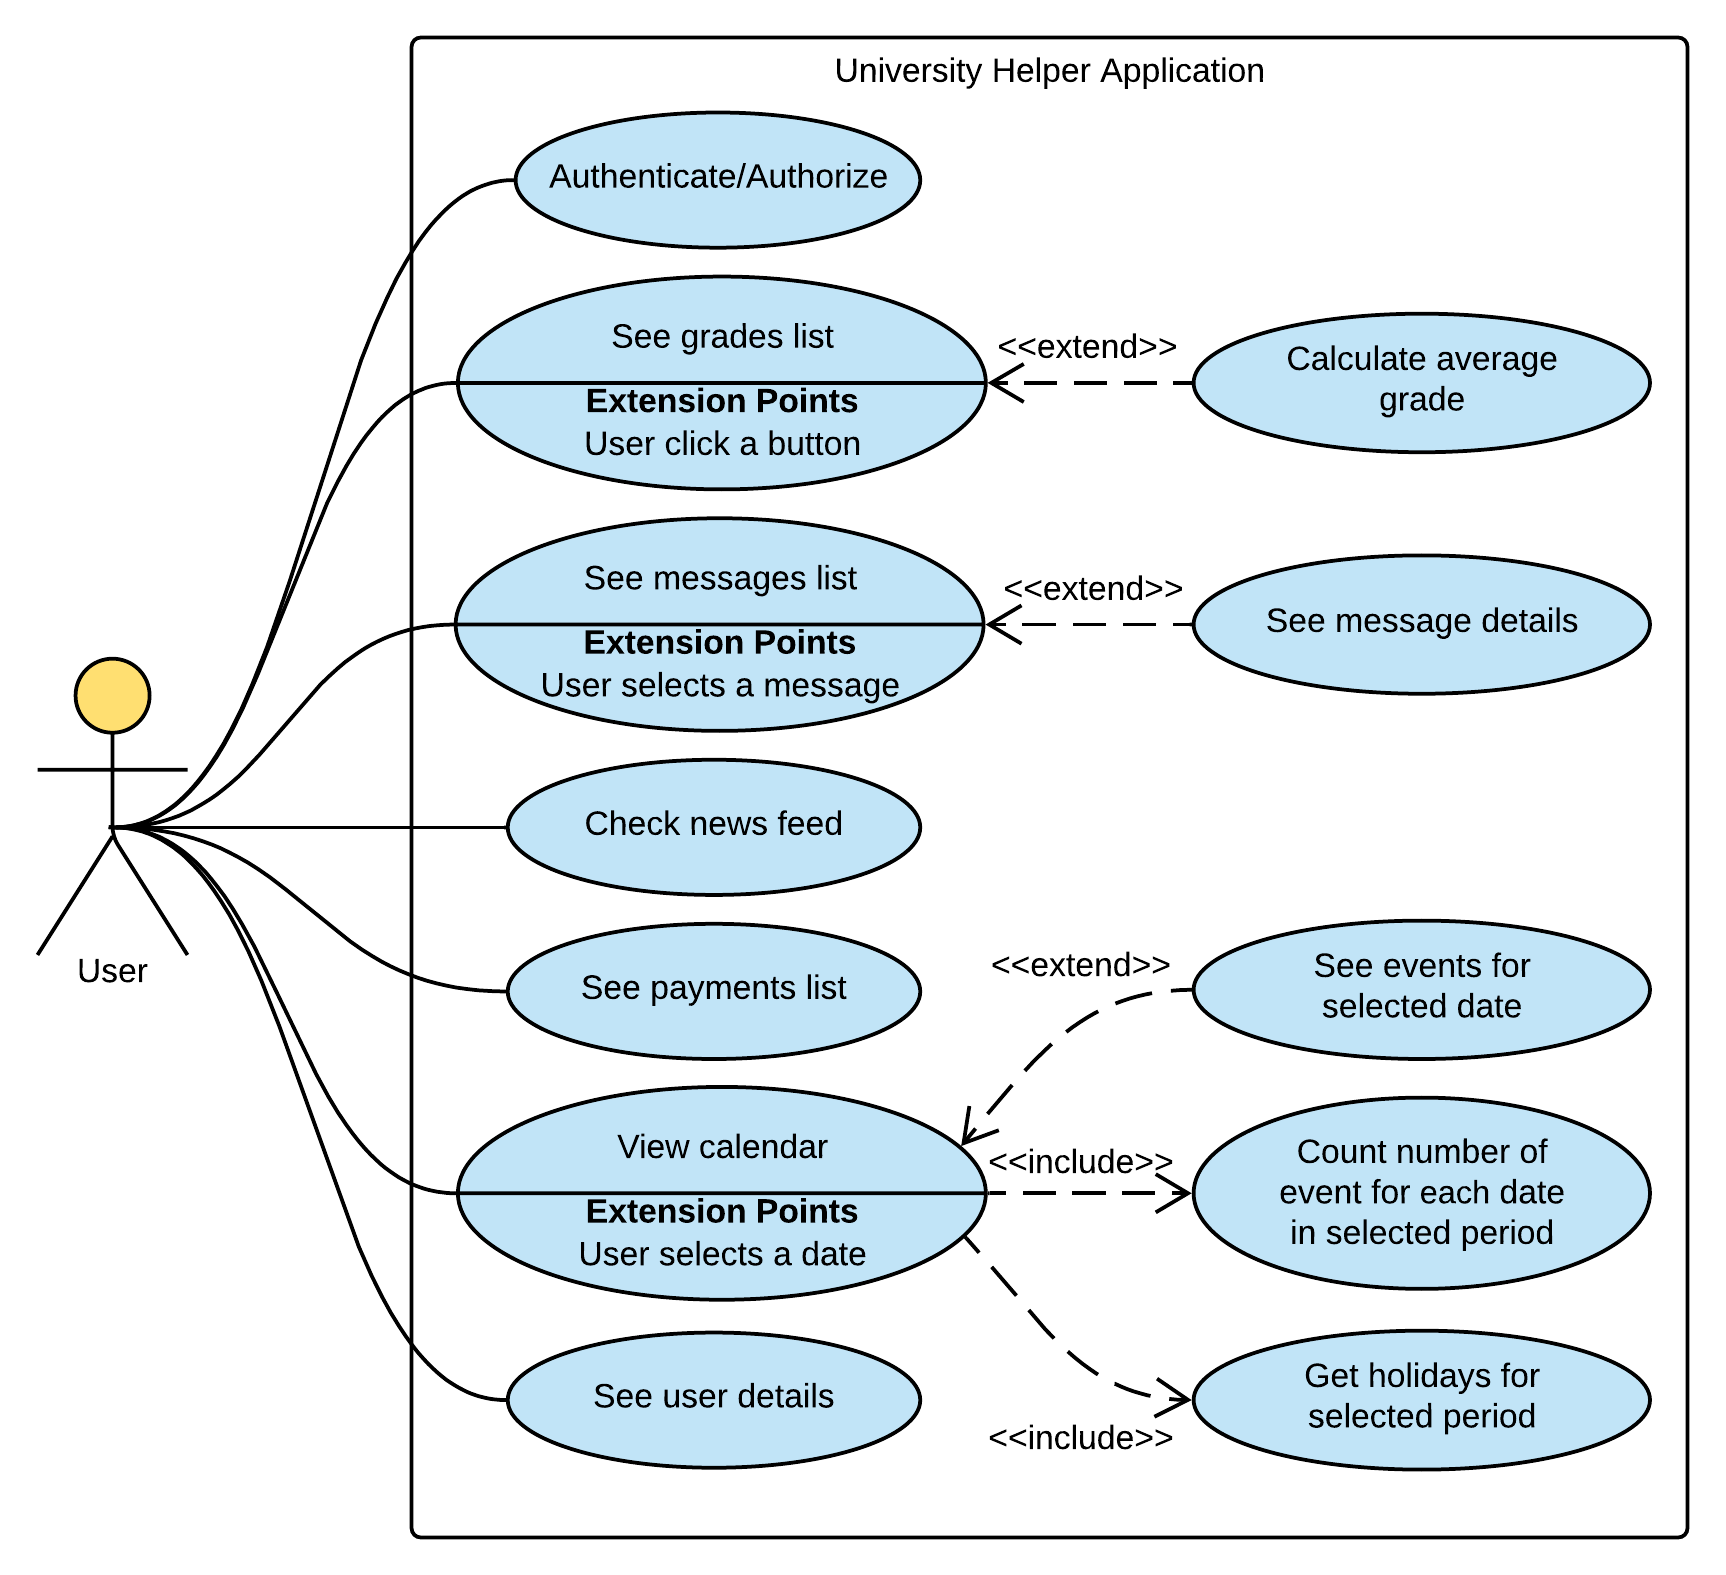
\includegraphics[width=0.93\textwidth]{fig02/use_case_diagram.png}
    \caption{Use case diagram} \label{fig:use-case-diagram}
\end{figure}

% ---------------------------------------------

\paragraph{\large{Authenticate/Authorize}}\mbox{}\\[2pt]
\textbf{Primary Actor:} User\\
\textbf{Scope:} Mobile application\\
\textbf{Level:} Fish level\\
\textbf{Brief:} The user logs in to the mobile application.\\
\textbf{Trigger:} The user open the mobile application.\\
\textbf{Preconditions:}
The user has an account in one of the available university systems.\\
\textbf{Basic flow:}
\begin{enumerate}
    \item The system's login screen has a drop-down with available universities.
    \item The user chooses her/his university and enter credentials.
    \item The user submits the form.
    \item The mobile application sends the credentials to the server.
    \item The server validates the credentials and sends a response back to the mobile application.
    \item The system redirects the user to the homepage.
\end{enumerate}
\textbf{Postconditions:}
The user is authenticated and can access all screens of the mobile application.

% ---------------------------------------------

\paragraph{\large{See grades list}}\mbox{}\\[2pt]
\textbf{Primary Actor:} User\\
\textbf{Scope:} Mobile application\\
\textbf{Level:} Sea level\\
\textbf{Brief:} The user wants to see her/his grades.\\
\textbf{Trigger:} The user selects "Grades" screen from the mobile application.\\
\textbf{Preconditions:}
\begin{itemize}
    \item The user has an account in one of the available university systems.
    \item The user is authenticated.
\end{itemize}
\textbf{Basic flow:}
\begin{enumerate}
    \item The system redirects the user to the "Grades" page.
    \item The mobile application sends a request to the server.
    \item The server fetches data from the university system and sends a response back to the mobile application.
    \item The mobile application loads the data and refreshes the view with the list of grades.
\end{enumerate}
\textbf{Postconditions:}
The user can see the list of her/his grades.\\
\textbf{Extensions:}
\begin{enumerate}[label=\alph*.]
    \item Calculate average grade:
    \begin{enumerate}
        \item The user clicks on the "Calculate average" button.
        \item The system calculates an average grade for all semesters and displays it to the user.
    \end{enumerate}
\end{enumerate}

% ---------------------------------------------

\paragraph{\large{See messages list}}\mbox{}\\[2pt]
\textbf{Primary Actor:} User\\
\textbf{Scope:} Mobile application\\
\textbf{Level:} Sea level\\
\textbf{Brief:} The user wants to see her/his messages.\\
\textbf{Trigger:} The user selects "Messages" screen from the mobile application.\\
\textbf{Preconditions:}
\begin{itemize}
    \item The user has an account in one of the available university systems.
    \item The user is authenticated.
\end{itemize}
\textbf{Basic flow:}
\begin{enumerate}
    \item The system redirects the user to the "Messages" page.
    \item The mobile application sends a request to the server.
    \item The server fetches data from the university system and sends a response back to the mobile application.
    \item The mobile application loads the data and refreshes the view with the list of messages.
\end{enumerate}
\textbf{Postconditions:}
The user can see the list of her/his messages.\\
\textbf{Extensions:}
\begin{enumerate}[label=\alph*.]
    \item See message details:
    \begin{enumerate}
        \item The user selects a message from the list.
        \item The system redirects the user to a page showing message details.
    \end{enumerate}
\end{enumerate}

% ---------------------------------------------

\paragraph{\large{See payments list}}\mbox{}\\[2pt]
\textbf{Primary Actor:} User\\
\textbf{Scope:} Mobile application\\
\textbf{Level:} Sea level\\
\textbf{Brief:} The user wants to see her/his payments.\\
\textbf{Trigger:} The user selects "Payments" screen from the mobile application.\\
\textbf{Preconditions:}
\begin{itemize}
    \item The user has an account in one of the available university systems.
    \item The user is authenticated.
\end{itemize}
\textbf{Basic flow:}
\begin{enumerate}
    \item The system redirects the user to the "Payments" page.
    \item The mobile application sends a request to the server.
    \item The server fetches data from the university system and sends a response back to the mobile application.
    \item The mobile application loads the data and refreshes the view with the list of payments.
\end{enumerate}
\textbf{Postconditions:}
The user can see the list of her/his payments.

% ---------------------------------------------

\paragraph{\large{Check news feed}}\mbox{}\\[2pt]
\textbf{Primary Actor:} User\\
\textbf{Scope:} Mobile application\\
\textbf{Level:} Sea level\\
\textbf{Brief:} The user wants to see news from her/his faculty and university.\\
\textbf{Trigger:} The user goes to the homepage of the mobile application.\\
\textbf{Preconditions:}
\begin{itemize}
    \item The user has an account in one of the available university systems.
    \item The user is authenticated.
\end{itemize}
\textbf{Basic flow:}
\begin{enumerate}
    \item The system redirects the user to the homepage.
    \item The mobile application sends a request to the server.
    \item The server fetches news from the university system and sends a response back to the mobile application.
    \item The mobile application loads the data and refreshes the news feed section.
\end{enumerate}
\textbf{Postconditions:}
The user can see the list of news in the news feed section of the homepage.

% ---------------------------------------------

\paragraph{\large{View calendar}}\mbox{}\\[2pt]
\textbf{Primary Actor:} User\\
\textbf{Scope:} Mobile application\\
\textbf{Level:} Sea level\\
\textbf{Brief:} The user wants to see her/his calendar.\\
\textbf{Trigger:} The user selects "Calendar" screen from the mobile application.\\
\textbf{Preconditions:}
\begin{itemize}
    \item The user has an account in one of the available university systems.
    \item The user is authenticated.
\end{itemize}
\textbf{Basic flow:}
\begin{enumerate}
    \item The system redirects the user to the "Calendar" page.
    \item The mobile application sends a request to the server.
    \item The server fetches data from the university system and sends a response back to the mobile application.
    \item The mobile application loads the data and refreshes the calendar with the list of events.
\end{enumerate}
\textbf{Postconditions:}
The user can see her/his calendar.
\textbf{Extensions:}
\begin{enumerate}[label=\alph*.]
    \item See events for selected date:
    \begin{enumerate}
        \item The user selects a date from the calendar.
        \item The system shows a list of events for the selected date.
    \end{enumerate}
\end{enumerate}

% ---------------------------------------------

\paragraph{\large{Get holidays for selected period}}\mbox{}\\[2pt]
\textbf{Primary Actor:} User\\
\textbf{Scope:} Mobile application\\
\textbf{Level:} Fish level\\
\textbf{Brief:} Get holidays from an external API for a selected period.\\
\textbf{Trigger:} The user selects "Calendar" screen from the mobile application or chooses another period.\\
\textbf{Preconditions:}
\begin{itemize}
    \item The user has an account in one of the available university systems.
    \item The user is authenticated.
\end{itemize}
\textbf{Basic flow:}
\begin{enumerate}
    \item The mobile application sends a request to the external API.
    \item The external API sends a response with a list of holidays for the selected period.
    \item The mobile application loads the data and refreshes the calendar with the list of holidays.
\end{enumerate}
\textbf{Postconditions:}
Holidays for the selected period are loaded into the system and shown on the calendar page.

% ---------------------------------------------

\paragraph{\large{Count number of event for each date in selected period}}\mbox{}\\[2pt]
\textbf{Primary Actor:} User\\
\textbf{Scope:} Mobile application\\
\textbf{Level:} Fish level\\
\textbf{Brief:} Count events for every date in the selected period.\\
\textbf{Trigger:} The user selects "Calendar" screen from the mobile application or chooses another period.\\
\textbf{Preconditions:}
\begin{itemize}
    \item The user has an account in one of the available university systems.
    \item The user is authenticated.
    \item The calendar events are stored in the system.
\end{itemize}
\textbf{Basic flow:}
\begin{enumerate}
    \item The mobile application loads events for each date in the selected period.
    \item The mobile application counts all events and refreshes the calendar with the number of events per day.
\end{enumerate}
\textbf{Postconditions:}
The number of events for each day in the selected period is shown on the calendar page.

% ---------------------------------------------

\paragraph{\large{See user details}}\mbox{}\\[2pt]
\textbf{Primary Actor:} User\\
\textbf{Scope:} Mobile application\\
\textbf{Level:} Sea level\\
\textbf{Brief:} The user wants to see profile details.\\
\textbf{Trigger:} The user goes to the homepage of the mobile application.\\
\textbf{Preconditions:}
\begin{itemize}
    \item The user has an account in one of the available university systems.
    \item The user is authenticated.
\end{itemize}
\textbf{Basic flow:}
\begin{enumerate}
    \item The system redirects the user to the homepage.
    \item The mobile application sends a request to the server.
    \item The server fetches user data from the university system and sends a response back to the mobile application.
    \item The mobile application loads the data and refreshes the profile info section.
\end{enumerate}
\textbf{Postconditions:}
The user can see the profile details section on the homepage.

\chapter{Project Design}
\section{System Architecture}

The system consists of two main components, as shown in Figure~\ref{fig:sys-architecture}. The first is the Flutter application, which is installed on the user's smartphone. On the first run, it will create a local SQLite database with the required tables. Whenever a user logs in or navigates to a page, it will send a request for data to the second component, the server. It is composed of configuration and transformation modules. The former is responsible for providing the YAML configuration file in the transformation application. Because both use Spring Cloud Config, the transformation application does not need to be restarted when the config changes. Each time it is updated, the configuration server will pick up the changes and serve the updated content. Now beans from the client that were using the configuration must be refreshed. A simple way to do this is to send a GET request to the "/ refresh" endpoint provided by the Spring Boot Actuator.

\begin{figure}[htb]
    \centering
    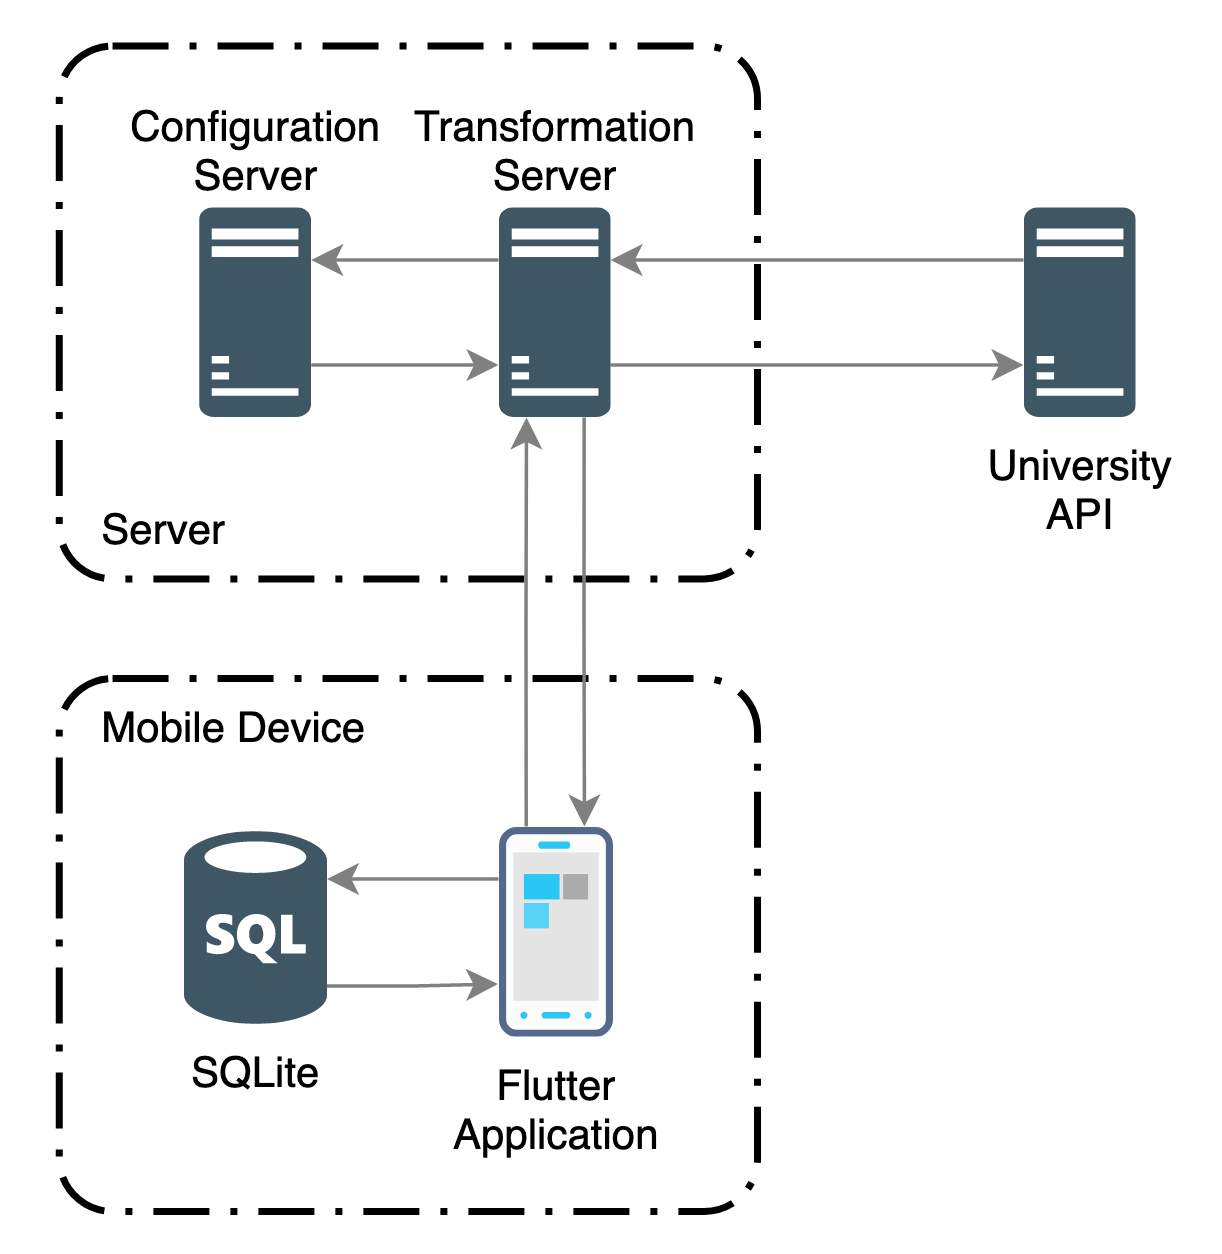
\includegraphics[width=0.55\textwidth]{fig03/system_architecture.png}
    \caption{System architecture}
    \label{fig:sys-architecture}
\end{figure}

When the transformation server receives a request, for example from Listing~\ref{list:login-request}, it reads the university and searches for a configuration for this particular institution.

\lstinputlisting[label=list:login-request,caption=Sample calendar request]{code03/calendar-request.json}

A sample YAML configuration for calendars is shown in Listing~\ref{list:calendar-config}. It contains an object with the name ``pwr'' and a configuration for this university. Every config entry has to contain a~name, endpoint address, a specification for Jolt transformation for request and response.

\lstinputlisting[label=list:calendar-config,caption=Sample YAML configuration for calendars]{code03/calendar-config.yml}

Every transformation operation requires a specification. Below is an example of conversion from one JSON schema (List.~\ref{list:json-input}) to another (List.~\ref{list:json-output}) using a JSON spec file (List.~\ref{list:json-spec}).

\lstinputlisting[label=list:json-input,caption=JSON transformation input]{code03/json-input.json}

\lstinputlisting[label=list:json-output,caption=JSON transformation output]{code03/json-output.json}

Operation type stated in the spec copies data from the input to the output tree without changing. Then we go inside the \texttt{events} array and get each entry with ``\texttt{*}''. The next step is to map \texttt{eventName} to \texttt{name} inside the output \texttt{events} array. Later we map \texttt{room} to \texttt{classroom} and \texttt{type} to \texttt{eventType}. Further, we go inside the \texttt{date} object and get \texttt{} and \texttt{end} and map it to \texttt{startDateTime} and \texttt{endDateTime} inside the output \texttt{events} array. The last action is to get the remaining, not mapped keys, and copy them into the \texttt{events} array.

\lstinputlisting[label=list:json-spec,caption=Transformation specification]{code03/json-spec.json}

\section{Database Design}
The mobile database is very straightforward. There are five separate tables as seen in Figure~\ref{fig:erd-diagram}. All of them are created during the first run of the application. Data received from the server is stored locally in the SQLite database. Every time the application sends a successful request, information in a chosen table is updated with new data. If there is no connection to the Internet, the app takes already stored details from the database instead of sending a request. Thanks to it, users can have constant access to data.
\begin{figure}[htb]
    \centering
    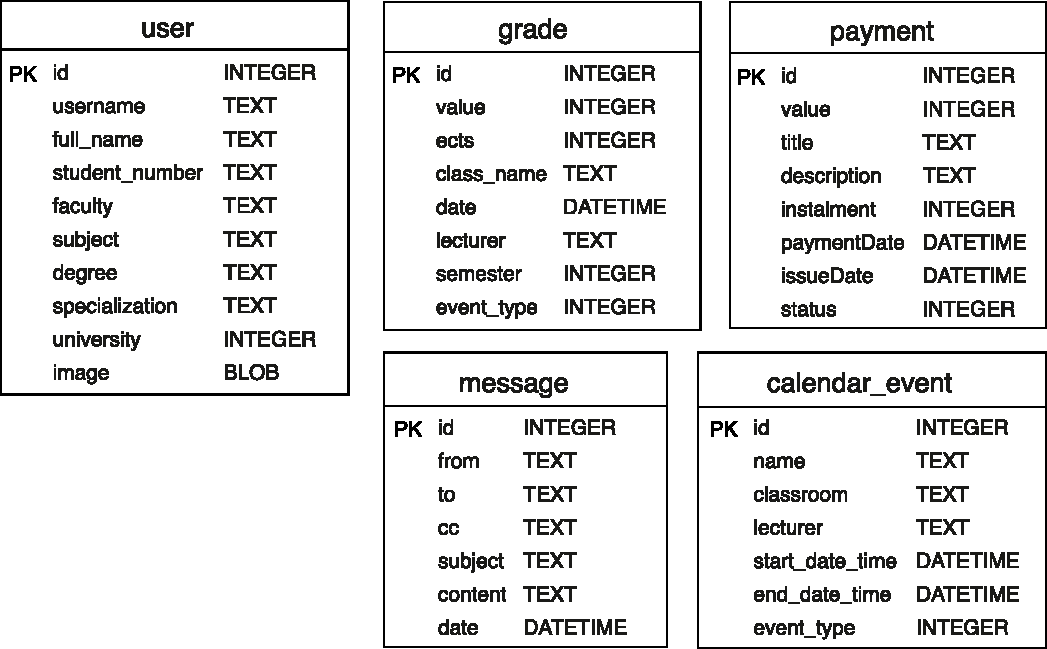
\includegraphics[scale=0.7]{fig03/erd_diagram.pdf}
    \caption{ERD diagram for the mobile database}
    \label{fig:erd-diagram}
\end{figure}

\section{User Interface Design}

All mobile applications should be easy to use and intuitive. In our app, we used Material Design~\cite{material-design} created by Google. It is also a part of the Flutter toolkit. To make the development quicker and easier, we created wireframes for all the main views of the application. To create them, we worked with a tool called Sketch~\cite{sketch}, which is simple to use and has a lot of available libraries.

Every mobile application requires a logo. To design a temporary one (Fig.~\ref{fig:app-logo}), we used a website created by FreeLogoDesign~\cite{freelogodesign}. It allows users to create logos by selecting templates and then customizing them using the built-in HTML5 wizard. It is free to use for low-resolution images, which was sufficient for our purpose.

\begin{figure}[htb]
    \centering
    
\includegraphics[scale=.9]{fig03/logo.png}
    \caption{Temporary logo}
    \label{fig:app-logo}
\end{figure}

There are seven main screens available with a navigation flow as shown in Figure~\ref{fig:ux-flow}. The first screen is a login screen. After users enter the correct login and password, they are redirected to the homepage. There they can see their profile info and news for their university and faculty. On the bottom, there is a navigation bar from which they can get access to an additional four pages. The first of them is the calendar page where they can see their schedule. The next one is the grades page where they can view all their grades. After it, there is the messages page where users can access their e-mails and go to the messages details page. The last one is the finances page. It allows users to see all of their payments.

\begin{figure}[htb]
    \centering
    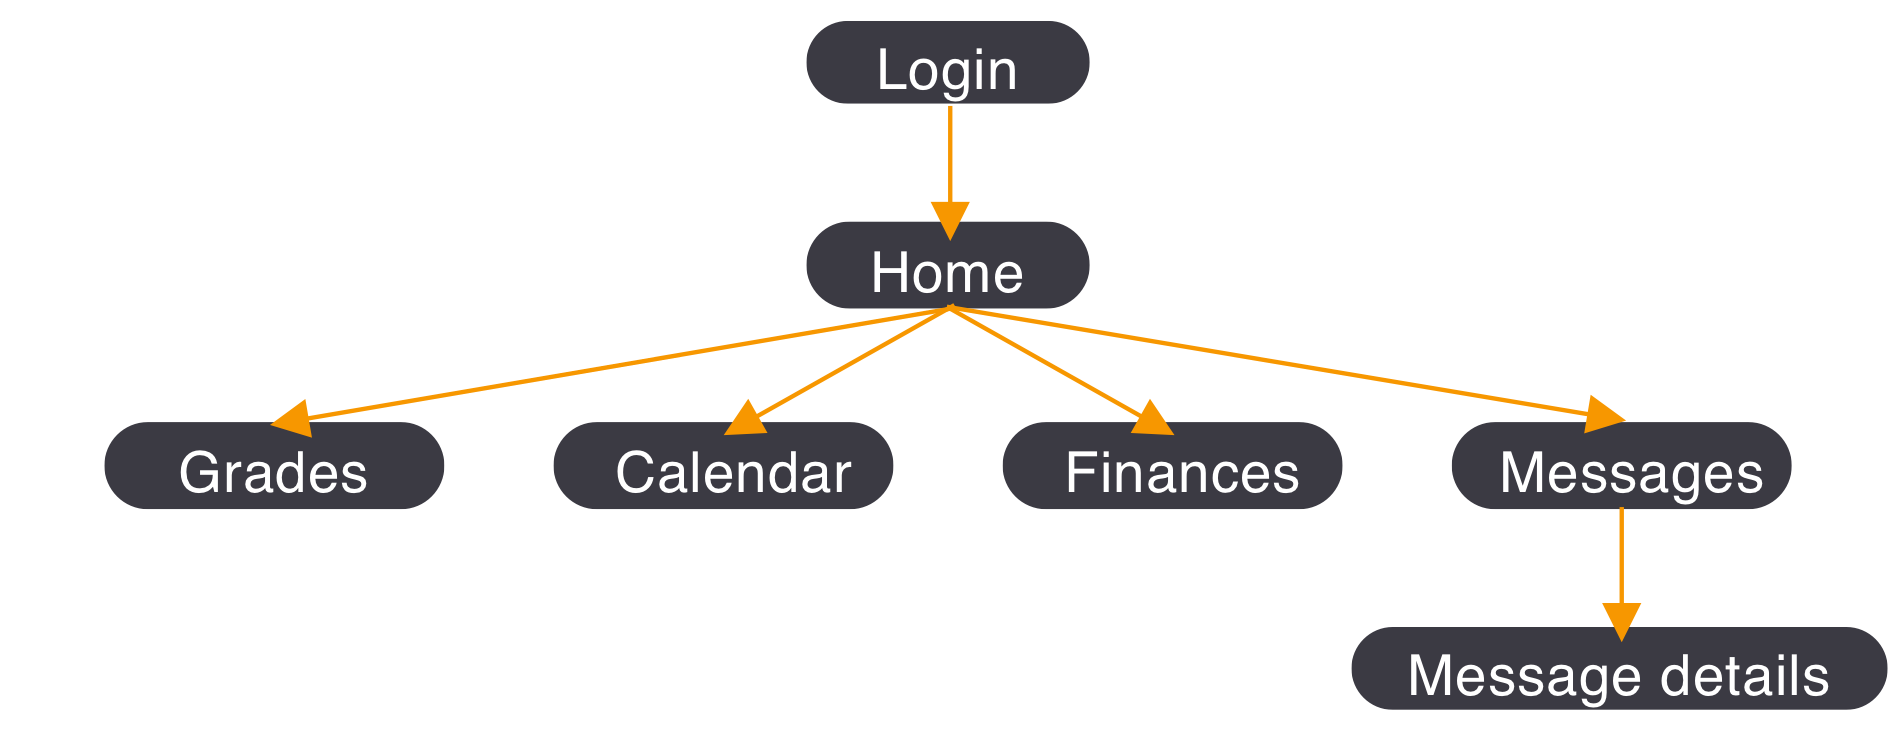
\includegraphics[width=0.6\textwidth]{fig03/mobile_ux_flow.png}
    \caption{Mobile UX flow}
    \label{fig:ux-flow}
\end{figure}

The first screen that is presented to users is the login screen (Fig.~\ref{fig:login-home}a). There is a big logo of the application in the middle of the view. There are also two input boxes on the bottom of the screen with a button to submit them. If the data provided is incorrect, users are presented with a red error snack bar.

The home screen (Fig.~\ref{fig:login-home}b), is the main page of the application. It contains profile info with the logged-in student's data. There is also a news feed section where users can access news from their university or faculty, depending on the configuration. In the top right corner of the screen, there are two icons. The first one allows users to log out of the application. By clicking on the next one, users can access the settings.

\begin{figure}[htb]
    \centering
    \begin{tabular}{@{}ll@{}}
        a) & b) \\
        {\setlength{\fboxsep}{0pt}\setlength{\fboxrule}{1pt}\fbox{\includegraphics[page=1,width=0.300\textwidth]{fig03/jsos_helper_wireframe.pdf}}} &
        {\setlength{\fboxsep}{0pt}\setlength{\fboxrule}{1pt}\fbox{\includegraphics[page=7,width=0.300\textwidth]{fig03/jsos_helper_wireframe.pdf}}} \\
    \end{tabular}
    \caption{Wireframes: a) login page, b) homepage} \label{fig:login-home}
\end{figure}

The calendar page (Fig.~\ref{fig:calendar-finances-grades}a) contains a calendar with the list of dates. If a date is a holiday, there is an indicator shown in the right top corner of the container. An indicator at the bottom of the container informs users that they have some lectures during the selected date.
When users click on a date, a list of classes is shown under the calendar. Every row contains the start and the end time of the event, its name, university teacher, classroom, and a type of the event.

The next screen (Fig.~\ref{fig:calendar-finances-grades}b) is the finances page. It is composed of a list of payments with their details. Every entry includes an amount, status, name, and the date of the payment's issue. Some of them also contain an installment number.

The last screen (Fig.~\ref{fig:calendar-finances-grades}c) consists of a grades list. Each entry contains a grade, number of ECTS credits, course name, type and university teacher, and issuing date. The icon in the top right corner allows users to calculate their average grade for a semester or the whole studies.

\begin{figure}[htb]
    \centering
    \begin{tabular}{@{}lll@{}}
        a) & b) & c) \\
        {\setlength{\fboxsep}{0pt}\setlength{\fboxrule}{1pt}\fbox{\includegraphics[page=2,width=0.300\textwidth]{fig03/jsos_helper_wireframe.pdf}}} &
        {\setlength{\fboxsep}{0pt}\setlength{\fboxrule}{1pt}\fbox{\includegraphics[page=6,width=0.300\textwidth]{fig03/jsos_helper_wireframe.pdf}}} &
        {\setlength{\fboxsep}{0pt}\setlength{\fboxrule}{1pt}\fbox{\includegraphics[page=3,width=0.300\textwidth]{fig03/jsos_helper_wireframe.pdf}}} \\
    \end{tabular}
    \caption{Wireframes: a) calendar page, b) finances page, c) the grades page} \label{fig:calendar-finances-grades}
\end{figure}

The two last screens shown in Figure~\ref{fig:messages-and-details} present a list of messages and their details. The first page is composed of the email sender, topic, date received, and partial contents. When customers click on an email, they are redirected to the details page where the full contents of the email are shown along with Cc'd recipients. After users have read the email, they can get back to the emails list by clicking an arrow on the top of the screen. In the top right corner of the screen, there is an icon that is shown only when the user university's API allows for sending messages.

\begin{figure}[htb]
    \centering
    \begin{tabular}{@{}ll@{}}
        a) & b) \\
        {\setlength{\fboxsep}{0pt}\setlength{\fboxrule}{1pt}\fbox{\includegraphics[page=4,width=0.300\textwidth]{fig03/jsos_helper_wireframe.pdf}}} &
        {\setlength{\fboxsep}{0pt}\setlength{\fboxrule}{1pt}\fbox{\includegraphics[page=5,width=0.300\textwidth]{fig03/jsos_helper_wireframe.pdf}}} \\
            \end{tabular}
    \caption{Wireframes: a) messages page, b) message details page} \label{fig:messages-and-details}
\end{figure}

\chapter{Project Design}
\section{System Architecture}

\begin{figure}[htb]
    \centering
    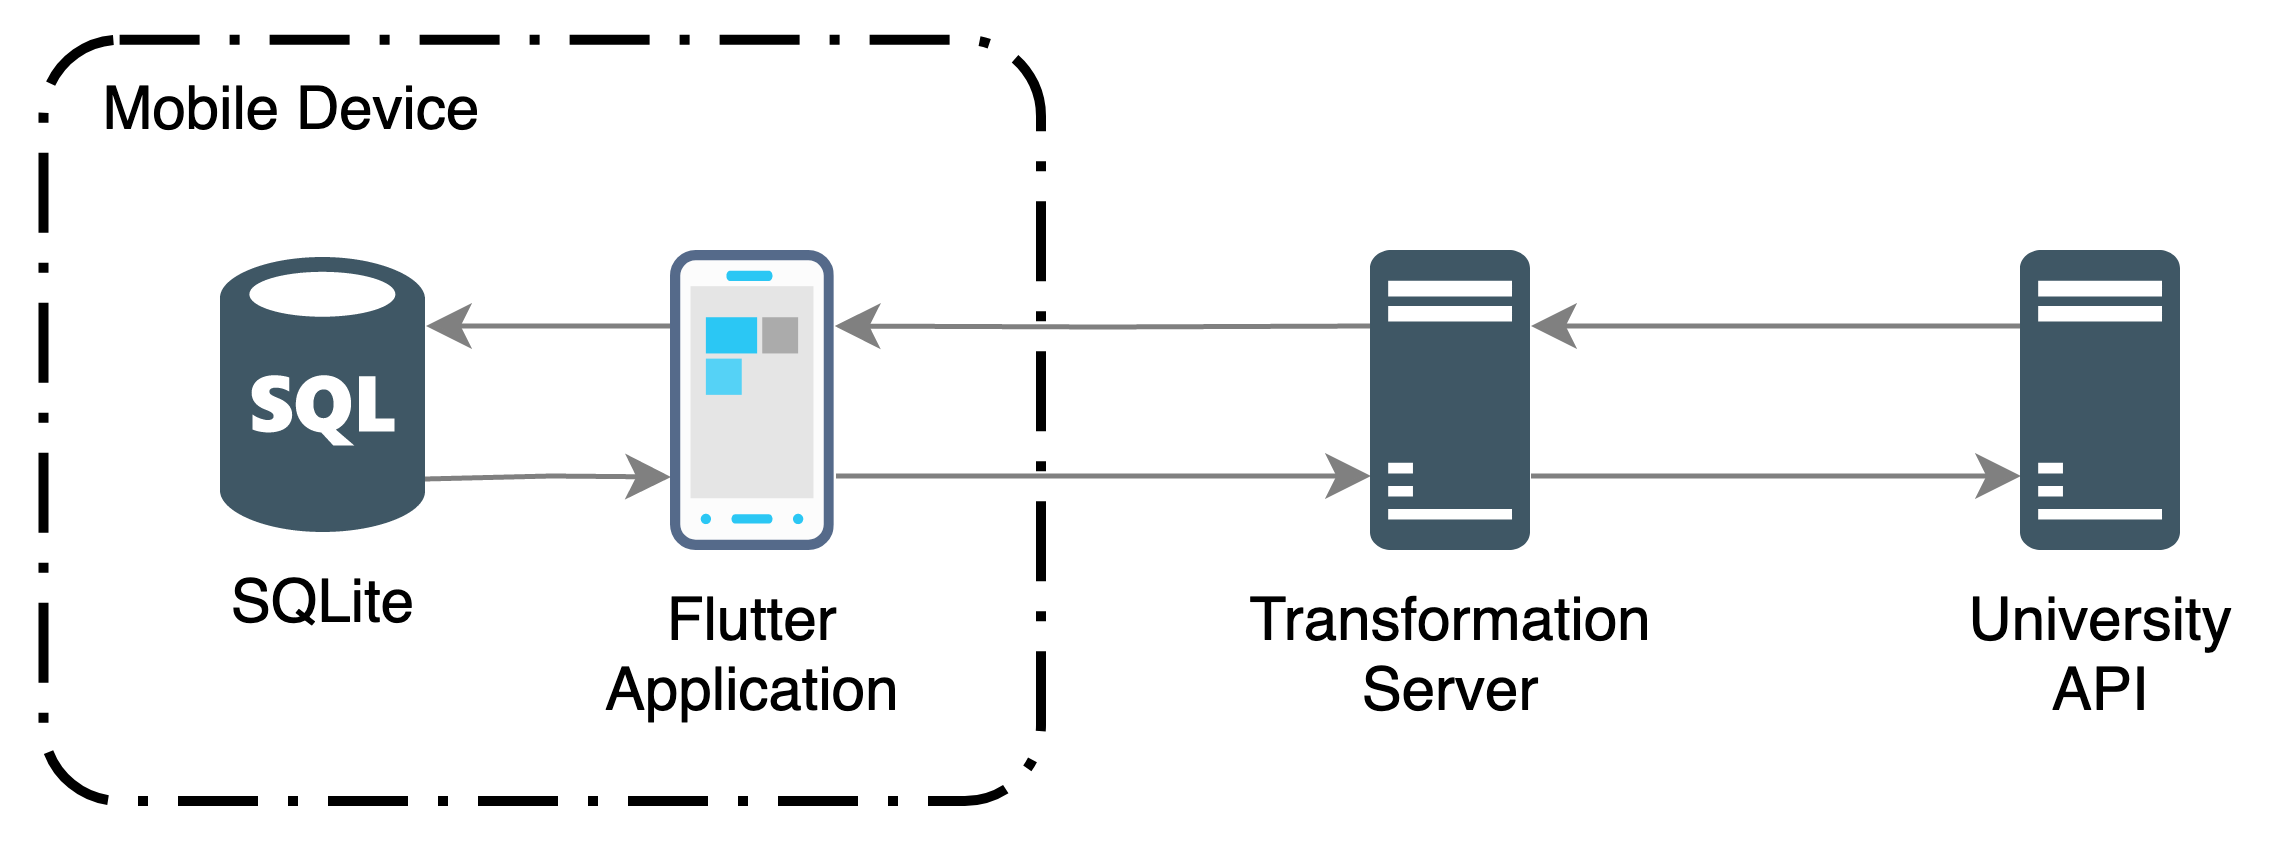
\includegraphics[width=0.66\textwidth]{fig04/system_architecture.png}
    \caption{System architecture}
    \label{fig:ux-flow}
\end{figure}

\section{Database Design}
\section{User Interface Design}

% TODO - ask what about Sketch, do I need a link or sth?
All mobile applications should be easy to use and intuitive. In our app, we used Material Design created by Google. It is also a part of the Flutter toolkit. To make the development quicker and easier, we created wireframes for all the main views of the application. To create them, we worked with a tool called Sketch, which is simple to use and has a lot of available libraries.

There are seven main screens available. All of them are shown in Figure~\ref{fig:ux-flow}. The first screen is a login screen. After users enter the correct login and password, they are redirected to the homepage. There they can see their profile info and news for their university and faculty. On the bottom, there is a navigation bar from which they can get access to an additional four pages. The first of the is the calendar page where they can see their schedule. The next one is the grades page where they can view all their grades. After it, there is the messages page where users can access their e-mails and go to the messages details page. The last one is the finances page. It allows users to see all of their payments.

\begin{figure}[htb]
    \centering
    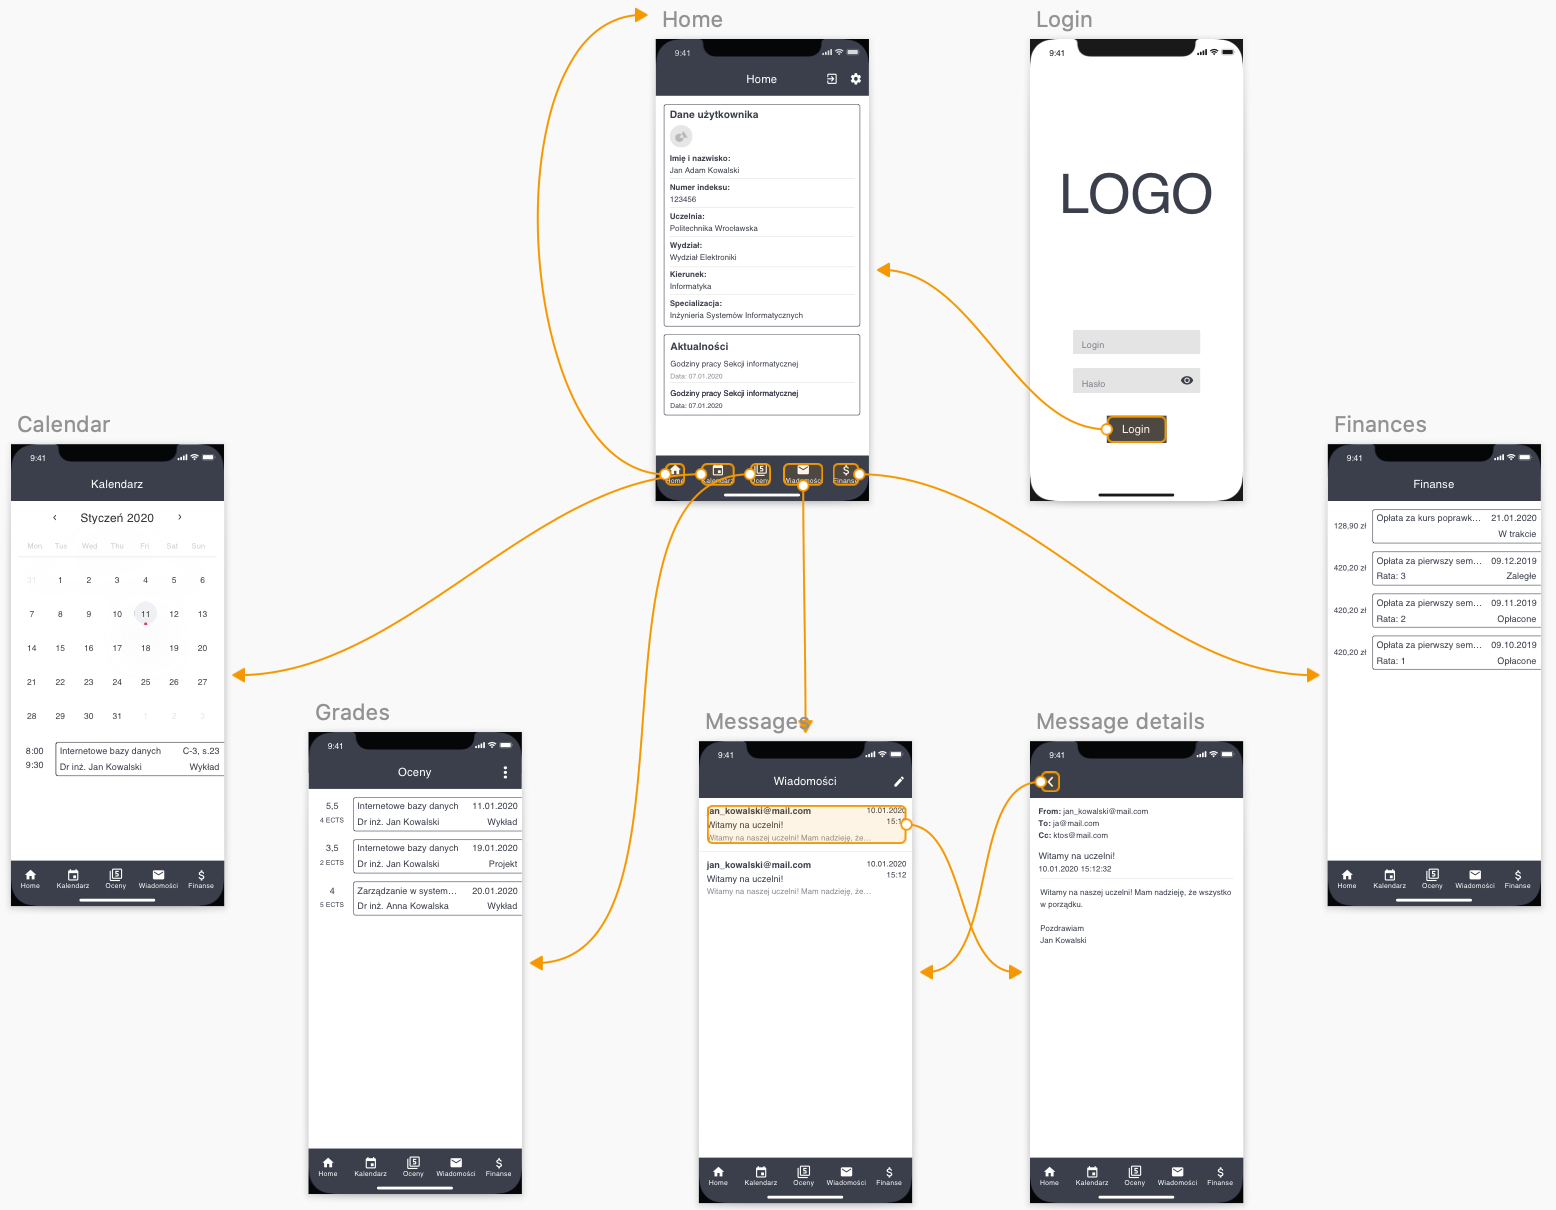
\includegraphics[width=\textwidth]{fig04/mobile_ux_flow.png}
    \caption{Mobile UX flow}
    \label{fig:ux-flow}
\end{figure}

The first screen that is presented to users is the login screen. It is shown in Figure~\ref{fig:login-home}. There is a big logo of the application in the middle of the view. There are also two input boxes on the bottom of the screen with a button to submit them. If the data provided is incorrect, users are presented with a red error snack bar.

The home screen, also presented in Figure~\ref{fig:login-home}, is the main page of the application. It contains profile info with the logged-in student's data. There is also a news feed section where users can access news from their university or faculty, depending on the configuration. In the top right corner of the screen, there are two icons. The first one allows users to log out of the application. By clicking on the next one, users can access the settings.

\begin{figure}[htb]
    \centering
    \begin{tabular}{@{}ll@{}}
        a) & b) \\
        \includegraphics[page=1,width=0.300\textwidth]{fig04/jsos_helper_wireframe.pdf} &
        \includegraphics[page=7,width=0.300\textwidth]{fig04/jsos_helper_wireframe.pdf} \\
    \end{tabular}
    \caption{Wireframes: a) login page, b) homepage} \label{fig:login-home}
\end{figure}

The calendar page shown in Figure~\ref{fig:calendar-finances-grades} contains a calendar with the list of dates. If a date is a holiday, there is an indicator shown in the right top corner of the container. An indicator at the bottom of the container informs users that they have some lectures during the selected date.
When users click on a date, a list of classes is shown under the calendar. Every row contains the start and the end time of the event, its name, university teacher, classroom, and a type of the event.

The next screen presented in Figure~\ref{fig:calendar-finances-grades} is the finances page. It is composed of a list of payments with their details. Every entry includes an amount, status, name, and the date of the payment's issue. Some of them also contain an installment number.

The last screen from Figure~\ref{fig:calendar-finances-grades} consists of a grades list. Each entry contains a grade, number of ECTS credits, course name, type and university teacher, and issuing date. The icon in the top right corner allows users to calculate their average grade for a semester or the whole studies.

\begin{figure}[htb]
    \centering
    \begin{tabular}{@{}lll@{}}
        a) & b) & c) \\
        \includegraphics[page=2,width=0.300\textwidth]{fig04/jsos_helper_wireframe.pdf} &
        \includegraphics[page=6,width=0.300\textwidth]{fig04/jsos_helper_wireframe.pdf} &
        \includegraphics[page=3,width=0.300\textwidth]{fig04/jsos_helper_wireframe.pdf} \\
    \end{tabular}
    \caption{Wireframes: a) calendar page, b) finances page, c) the grades page} \label{fig:calendar-finances-grades}
\end{figure}

The two last screens shown in Figure~\ref{fig:messages-and-details} present a list of messages and their details. The first page is composed of the email sender, topic, date received, and partial contents. When customers click on an email, they are redirected to the details page where the full contents of the email are shown along with Cc'd recipients. After users have read the email, they can get back to the emails list by clicking an arrow on the top of the screen. In the top right corner of the screen, there is an icon that is shown only when the user university's API allows for sending messages.

\begin{figure}[htb]
    \centering
    \begin{tabular}{@{}ll@{}}
        a) & b) \\
        \includegraphics[page=4,width=0.300\textwidth]{fig04/jsos_helper_wireframe.pdf} &
        \includegraphics[page=5,width=0.300\textwidth]{fig04/jsos_helper_wireframe.pdf} \\
            \end{tabular}
    \caption{Wireframes: a) messages page, b) message details page} \label{fig:messages-and-details}
\end{figure}

% \section{Server Architecture}

% Do implementation
\section{Wzorce projektowe}
BLOC, MVVM
\section{Zarządzanie projektem}
glo, git flow
\chapter{Project Tests}
\section{Mobile Application Tests}
\subsection{Unit Tests}
A unit test tests a single class, method, or function~\cite{testing-flutter}. The purpose of the unit test is to check the correctness of a logical unit under various conditions. External dependencies of the tested unit are usually mocked out. Unit tests generally do not render to screen, read from, or write to disk, or receive user actions from outside of the process running the test.

An example of such a test is shown in Listing~\ref{list:login-bloc-test}. First, we have to mock the \texttt{UserRepository} and \texttt{AuthenticationBloc} to eliminate any distortions. In the \texttt{setUp} method, we instantiate a new instance of \texttt{AuthenticationBloc} to ensure that each test runs under the same conditions and does not affect subsequent tests. The \texttt{tearDown} method runs after each test and destroys all unused objects. Next is a group of tests that imitates a user pressing the login button. First, we set the expected response, which consists of three states. In the end, we expect that the \texttt{LoginBloc} will yield \texttt{LoginInitial}, followed by a \texttt{LoginLoading} and lastly a \texttt{LoginInitial} in response to the \texttt{LoginButtonPressed} event.

\lstinputlisting[label=list:login-bloc-test,caption=Flutter login BLoC test]{code05/login_bloc_test.dart}

\subsection{Widget Tests}
A widget test (sometimes called the component test) tests a single widget~\cite{testing-flutter}. The goal of it is to check that the widget's UI looks and interacts as expected. Testing a widget involves many classes and requires a test environment that provides the appropriate widget life cycle context.

For instance, widgets that are being tested should be able to receive and respond to user events and actions, perform layout, and instantiate child widgets. This kind of test is more comprehensive than a unit test. Though, like unit tests, a widget tests' environment is replaced with an implementation much more straightforward than a fully developed UI system.

Two examples of widget tests are shown in Listing~\ref{list:widget-test}. First, we need to create a \texttt{CustomCard} widget that will be tested in the next steps. The component is responsible for rendering items in grades and payments lists (see Fig~\ref{fig:calendar-finances-grades}). The \texttt{buildTestableWidget} method wraps the widget with the \texttt{MaterialApp} and \texttt{MediaQuery} so that it can be built and tested correctly.

The next part checks if the ``CustomCard widget has aside, right and left widgets''. First, we have to build \texttt{CustomCard} inside the test environment by using the \texttt{pumpWidget} method provided by WidgetTester. It builds and renders the provided widget.

The following steps use the \texttt{find} method to search through the widget tree for the aside, right, and left widget. Then, as a result, we expect to locate one \texttt{asideWidget}, two \texttt{rightWidget}s, and one \texttt{leftWidget} component. The test ends successfully if all expected values match what has been found by using \texttt{Finder}.

The second test also uses the \texttt{CustomCard} type. It verifies that the ``CustomCard widget has a color''. First, we have to build the component, and then we can create a predicate used to filter widgets. We want to find only components that are \texttt{Containers} and have a decoration attribute equal to the specified \texttt{BoxDecoration}. If such components are found, the test passes.

\lstinputlisting[label=list:widget-test,caption=Flutter widget tests]{code05/widget_test.dart}

\section{Server Application Tests}
The transformation server required some manual testing when creating the configuration YAML files. All of it was done from the Postman application~\cite{postman}. A sample POST request to fetch calendar data shown in Listing~\ref{list:calendar-request} was used to test the transformation configuration.

\begin{lstlisting}[label=list:calendar-request,caption=Sample content of the POST request to fetch calendar data]
{
	"university": "pwr",
	"username": "pwr230115",
	"studentNumber": "123456",
	"startDate": "2020-01-01",
	"endDate": "2020-01-31"
}
\end{lstlisting}

Apart from the manual testing, the transformation was validated by unit tests. One of them is demonstrated below (List.~\ref{list:transformation-service-test}) and checks if the function responsible for translating all incoming requests and responses works as expected. It is a Spring Boot test, as indicated by the \texttt{@SpringBootTest} annotation. At the top of the \texttt{TransformationServiceTest} class are the static strings used to prepare the tests:
\begin{itemize}
    \item \texttt{REQUEST\_SPEC} - Jolt specification for the request;
    \item \texttt{RESPONSE\_SPEC} - Jolt specification for the response;
    \item \texttt{ADDRESS} - the API endpoint;
    \item \texttt{UNIVERSITY} - the chosen university;
    \item \texttt{CALENDAR\_JSON\_INPUT} - sample calendar request;
    \item \texttt{CALENDAR\_JSON\_OUTPUT} - expected calendar response.
\end{itemize}

\texttt{@BeforeAll} annotation placed above the \texttt{initAll} indicates that the method executes only once, before any test function. Inside it, a new transformation is initialized using predefined static strings.

The last method, called \texttt{transformCalendarJson}, tests the \texttt{transformJson} method from the \texttt{transformationService} class, which was autowired at the beginning. The \texttt{output} variable stores the result of the JSON transformation, which is compared, int the end, with the expected output. If they are equal, the test passes, if they are not the same or there was an exception while creating a new \texttt{JSONObject}, the test fails.

\lstinputlisting[label=list:transformation-service-test,caption=Tests for the transformation service requests]{code05/TransformationServiceTest.java}

\chapter{Project Presentation}
The created application runs on both iOS and Android devices. It was installed only on one real device, iPhone XS, and it worked as expected. The iOS device simulation included in Xcode~\cite{xcode} is very accurate, and it well illustrates the final look of the app. All screenshots shown in this chapter were created using the iOS simulator. The main reason for that is that all testing data has been prepared on a local machine, including data in the SQLite database and mocked university API. The transformation server and its configuration have not been deployed to any external server, so they both have to be run locally.

Two images shown in Figure~\ref{fig:login-dropdown} represent the login screen in two states. The first one is the basic page with a university drop-down menu and two input fields for user login and password. The next image depicts the previous screen with the expanded university drop-down.

\begin{figure}[b]
    \centering
    \begin{tabular}{@{}l@{}l@{}l@{}l@{}}
        a) & \vtop{\vskip-2ex\hbox{{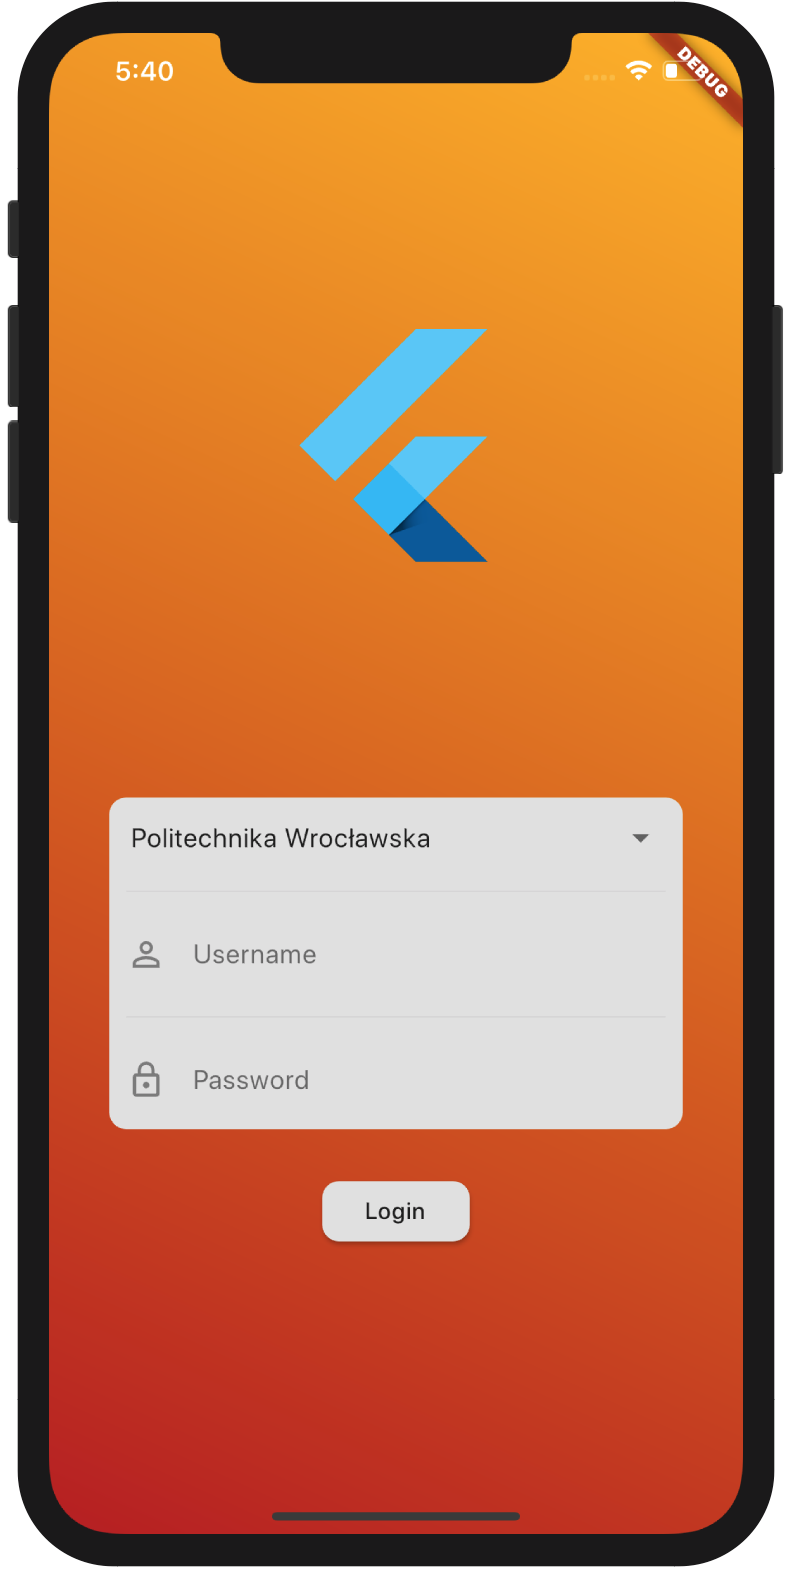
\includegraphics[page=1,width=0.3\textwidth]{fig06/login_page.png}}}} &
        b) & \vtop{\vskip-2ex\hbox{{\includegraphics[page=7,width=0.3\textwidth]{fig06/login_page_dropdown.png}}}} \\
    \end{tabular}
    \caption{Screenshots of the mobile application: a) login page, b) login page with the university drop-down menu} \label{fig:login-dropdown}
\end{figure}

The screen seen by users after they log in is the homepage (Fig.~\ref{fig:home-grades-payments}a). At the top, there are two icons (logout and settings). When users click on the first one, they get logged out of the app. The second one should open a settings tab where users could change some properties. It has not been implemented yet. Also, the default application language is set to English. As of now, the language change functionality has not been implemented.

In the middle, there is a ``Profile'' section where users can see their details like name, student number, university, degree, faculty, subject, and specialization. This segment also contains a user profile photo retrieved from the system. The next area consists of news from users' faculty and university websites.
All screens, except the login page, have bottom navigation. It allows users to change tabs and quickly see which page they are currently on.

The page shown in Figure~\ref{fig:home-grades-payments}b lists all user grades with their details. On the left side, there is a section with the grade value and number of ECTS credits associated with the class. On the right, starting from the top, there is the class name, date of issue, lecturer, and type of class.

The screen presented in  Figure~\ref{fig:home-grades-payments}c shows a list of payments related to the current user. Each entry has a value (in Polish złotys), name, date of payment, and status. The number of the installment is an optional property and does not have to occur in every element.

\begin{figure}[t]
    \centering
    \begin{tabular}{@{}l@{}l@{}l@{}l@{}l@{}l@{}}
        a) & \vtop{\vskip-2ex\hbox{{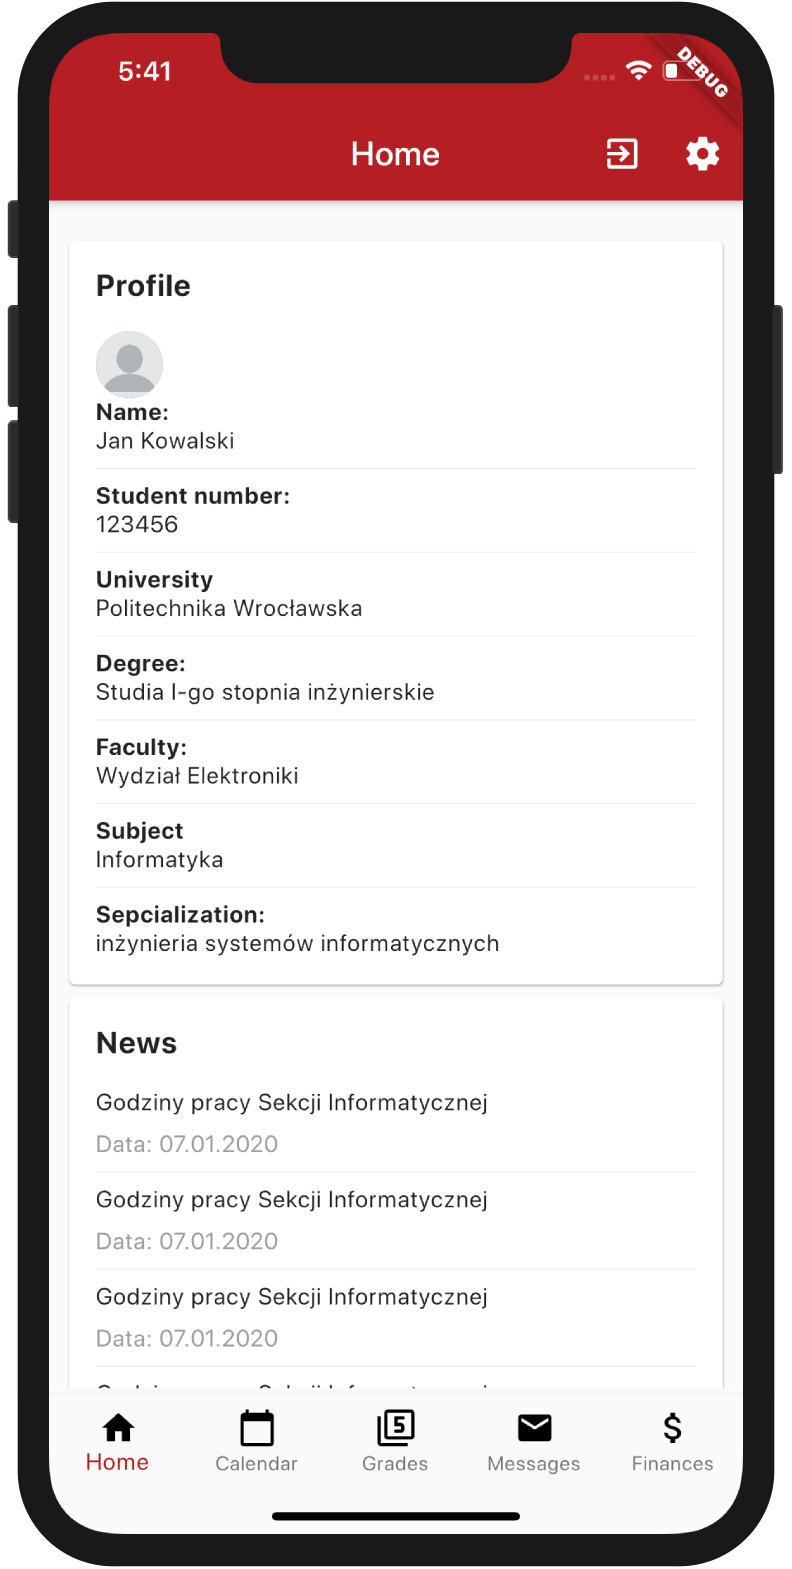
\includegraphics[page=1,width=0.3\textwidth]{fig06/home_page.png}}}} &
        b) & \vtop{\vskip-2ex\hbox{{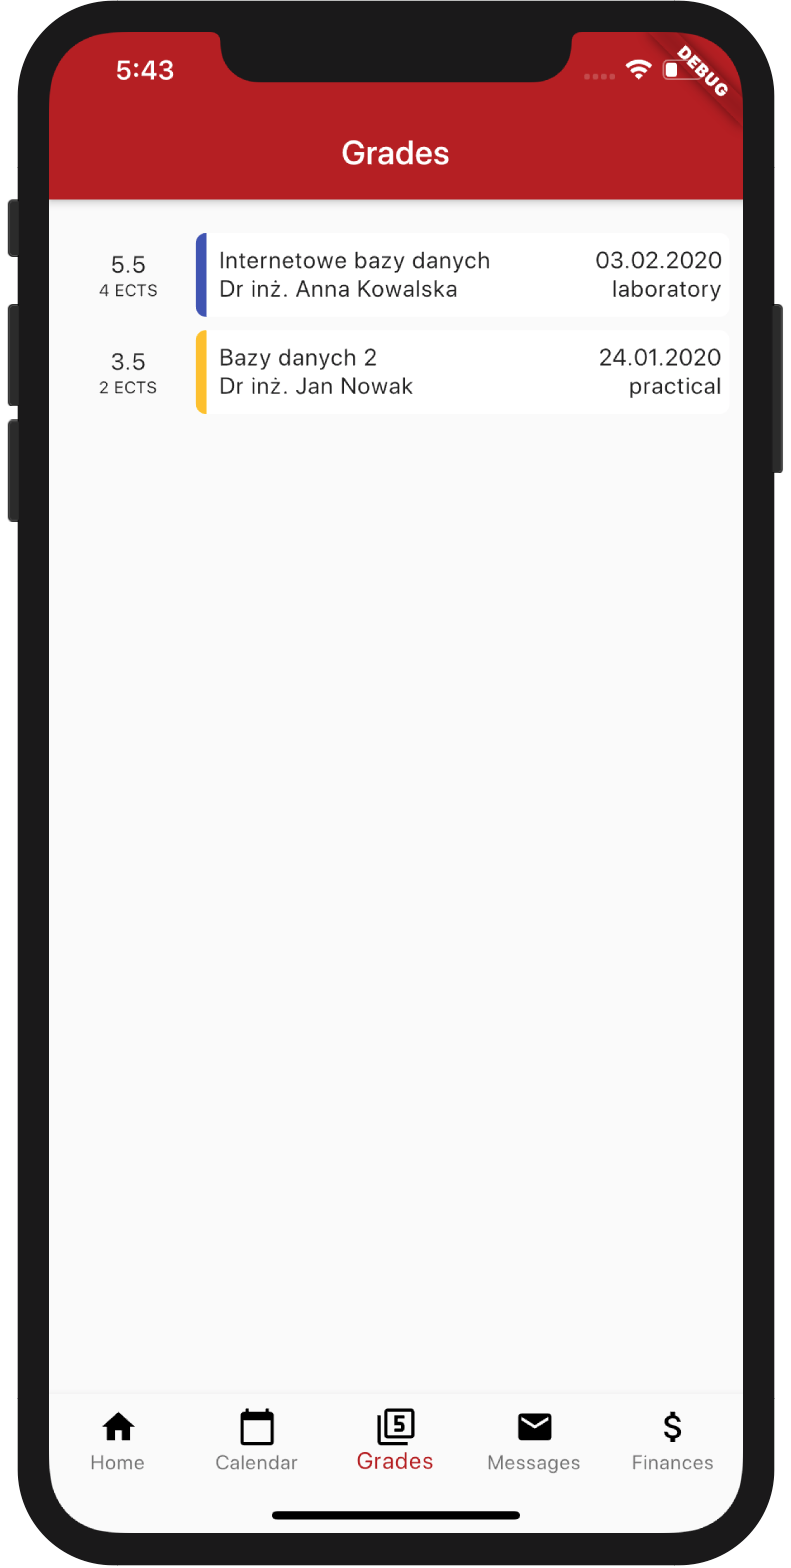
\includegraphics[page=1,width=0.3\textwidth]{fig06/grades_page.png}}}} &
        c) & \vtop{\vskip-2ex\hbox{{\includegraphics[page=7,width=0.3\textwidth]{fig06/payments_page.png}}}} \\
    \end{tabular}
    \caption{Screenshots of the mobile application: a) homepage, b) grades page, c) payments page} \label{fig:home-grades-payments}
\end{figure}

One of the most important screens in the application is the calendar page (Fig.~\ref{fig:calendar-page}). It shows all classes that the user have to attend. The first image (Fig.~\ref{fig:calendar-page}a) does not present any events planned for the selected date. All red numbers indicate that it is a weekend or a holiday. The house at the top right corner means that the university is not working and the user can stay at home instead of going to class.
\begin{figure}[t]
    \centering
    \begin{tabular}{@{}l@{}l@{}l@{}l@{}}
        a) & \vtop{\vskip-2ex\hbox{{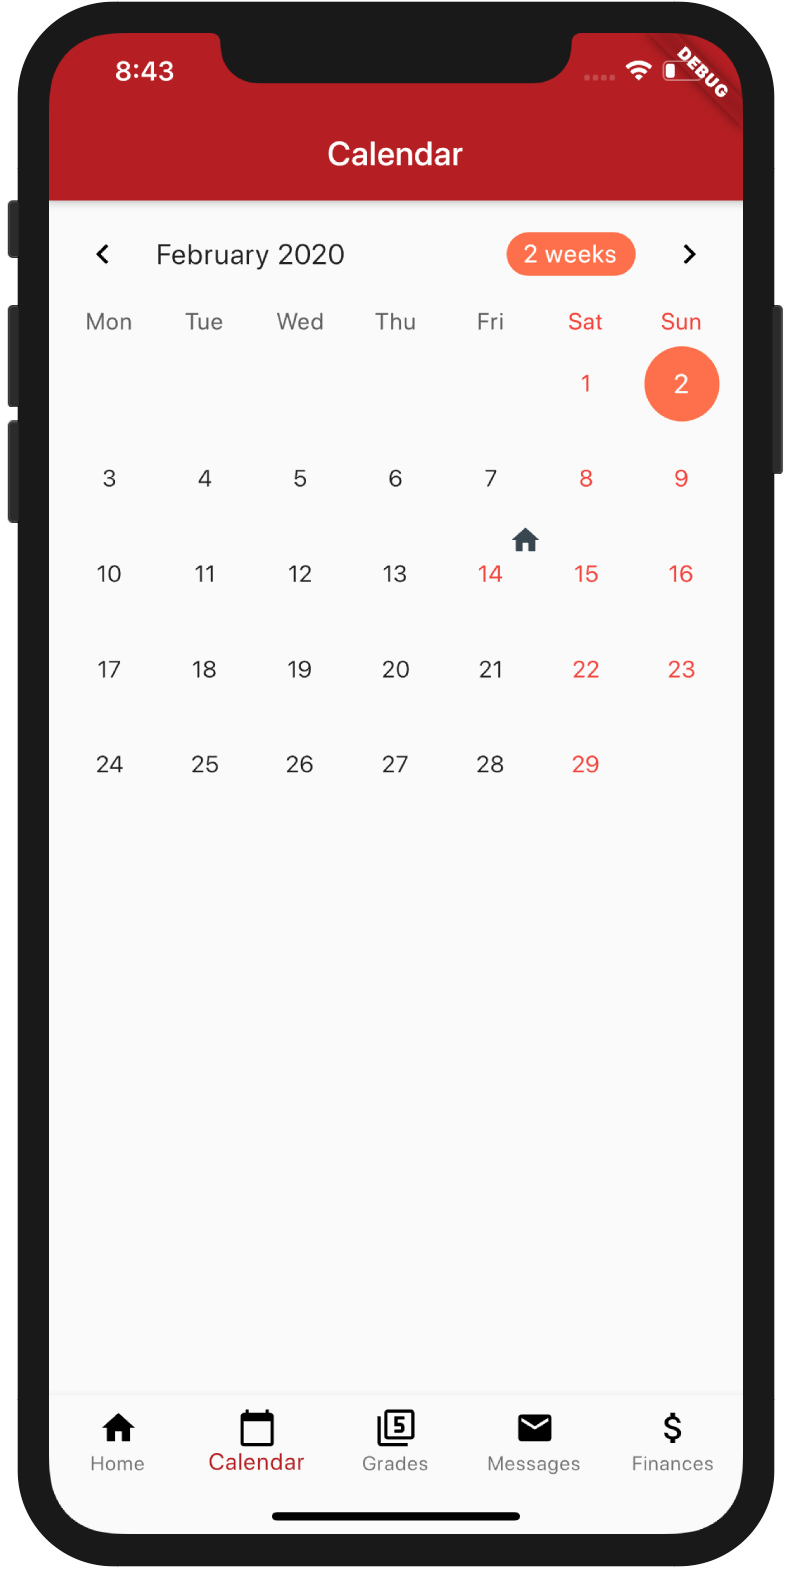
\includegraphics[page=1,width=0.3\textwidth]{fig06/calendar_page_no_classes.png}}}} &
        b) & \vtop{\vskip-2ex\hbox{{\includegraphics[page=7,width=0.3\textwidth]{fig06/calendar_page_with_classes.png}}}} \\
    \end{tabular}
    \caption{Screenshots of the mobile application: a) calendar page with no classes, b) calendar page with available classes} \label{fig:calendar-page}
\end{figure}

The image in Figure~\ref{fig:calendar-page}b shows a different view of the calendar. It can be swapped using the button in the top right corner of the page. There are three available appearances:
\begin{itemize}
    \item one month;
    \item 2 weeks;
    \item a week.
\end{itemize}
 
The indicator in the lower-left corner of a day tells users how many events they have planned. When users select a date, a list of classes appears with details such as the beginning and the end of the class, its name, lecturer, classroom, and type.
The viewed month can be changed by swapping the screen left or right or by clicking on one of the arrows at the top of the page.


The messages page (Fig.~\ref{fig:messages-details-page}a) lists all messages received by users in their university system. On the left-hand side, there is a section displaying specifics like sender, topic, and partial content. On the right, there is a date of receipt. After users select one of the listed messages, they are redirected to a more detailed page (Fig.~\ref{fig:messages-details-page}b) where they can view, in addition to previously seen details, the entire content of the message, and CC recipients.
\begin{figure}[hb]
    \centering
    \begin{tabular}{@{}l@{}l@{}l@{}l@{}}
        a) & \vtop{\vskip-2ex\hbox{{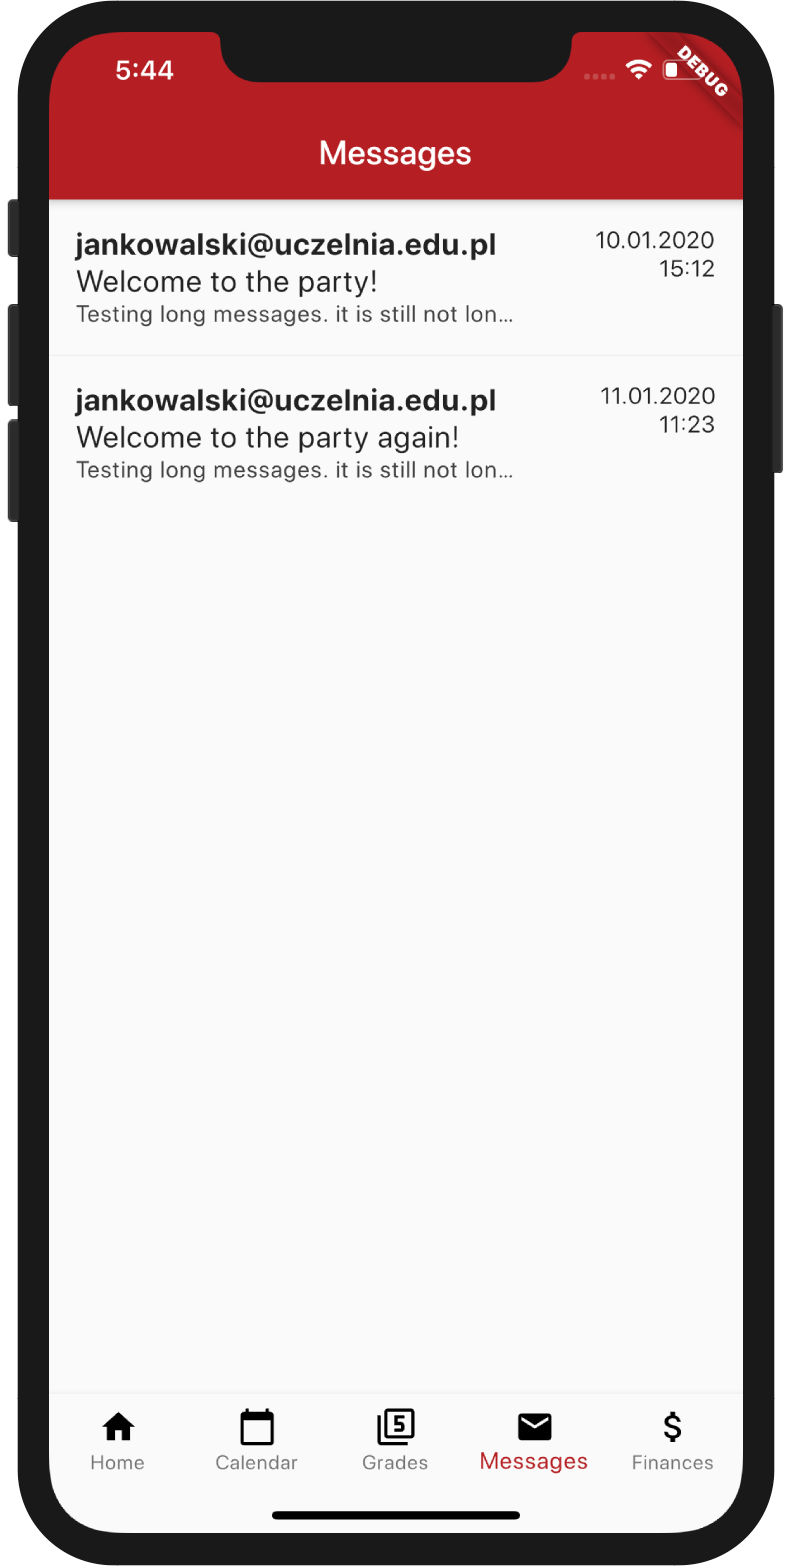
\includegraphics[page=1,width=0.3\textwidth]{fig06/messages_page.png}}}} &
        b) & \vtop{\vskip-2ex\hbox{{\includegraphics[page=7,width=0.3\textwidth]{fig06/message_details_page.png}}}} \\
    \end{tabular}
    \caption{Screenshots of the mobile application: a) messages page, b) message details page} \label{fig:messages-details-page}
\end{figure}


%\bibliographystyle{plalpha}
\bibliographystyle{plabbrv}
% \bibliographystyle{plain}

%UWAGA: bibliotekę referencji należy przygotować samemu. Dobrym do tego narzędziem jest JabRef.
%       Nazwę przygotowanej biblioteki wpisuje się poniżej bez rozszerzenia 
%       (w tym przypadku jest to "dokumentacja.bib")
\bibliography{bibliography}
\appendix
\chapter{Description of the attached CD/DVD}
The attached disk contains code and builds of the created applications (Fig~\ref{fig:directory structure}). The \texttt{mobile} directory contains \texttt{code} and \texttt{release} folders. Inside the first one is the source code of the Flutter mobile application with license and readme files. The second one holds Android application packages (APK) for three different architectures (\texttt{app-arm64-v8a-release.apk}, \texttt{app-armeabi-v7a-release.apk}, \texttt{app-x86\_64-release.apk}), as well as a build dedicated to iOS devices (\texttt{jsos\_helper.app}). All of them can be run on a smartphone or a computer using emulation software.

\begin{figure}[htb]
    \footnotesize{\ttfamily{
        \dirtree{%
        .1 root.
        .2 mobile.
        .3 code.
        .4 ....
        .3 release.
        .4 app-arm64-v8a-release.apk.
        .4 app-armeabi-v7a-release.apk.
        .4 app-x86\_64-release.apk.
        .4 jsos\_helper.app.
        .2 server.
        .3 code.
        .4 ....
        .3 release.
        .4 docker-compose.yml.
        .4 mockserver-config.
        .5 initializerJson.json.
        .5 mockserver.properties.
        .4 transformation-config.
        .5 university-helper-server.yml.
        .4 university-helper-server-client-1.0.0.jar.
        .4 university-helper-server-config-1.0.0.jar.
        }
    }}
    \caption{Disk directory structure} \label{fig:directory structure}
\end{figure}

The server subtree contains the \texttt{code} folder with the source code of the translation and configuration modules. Inside the parent project, there are license and readme files. In the \texttt{release} folder, there is the \texttt{docker-compose.yml} file for running the entire server and the mocking service at once. The \texttt{mockserver-config} holds MockService startup configuration. The \texttt{transformation-config} stores Spring Cloud Config properties used to translate JSON schemas. Last but not least, there are two jars (\texttt{university-helper-server-client-1.0.0.jar}, \texttt{university-helper-server-config-1.0.0.jar}), one for each server module.

\chapter{System Deployment}
The mobile application can be installed from the attached APK files for Android devices. To do so, we need to copy a package for the chosen architecture onto a smartphone. Then we only have to click on the copied application and let it install on the device. Installing the iOS package is more complicated, so it is much better to run it in an XCode simulator instead of a mobile machine. We simply have to start the virtual device and drag and drop our package onto its screen. The Android application can also be run on an Android emulator.

In the case of this project, it is best to run it on a computer instead of a mobile device. We use MockServer to mimic the behavior of a real student services system API. The mock server is not embedded into the mobile application, and because of this, logging in and browsing screens is not possible for applications installed on smartphones.

The best way to test this proof of concept is to run the mobile application using an Android or iOS emulator and start the backend server using the steps described below.

Docker and Docker Compose were used to simplify the startup of the server application and the API mocking service. Both tools are required for the next steps, so they must be installed on the system. To start the whole backend, we need to run the following commands from the disk root directory:
\begin{lstlisting}[numbers=none]
cd server/release
docker-compose up
\end{lstlisting}

\noindent You can also run and stop Docker in the detached mode:
\begin{lstlisting}[numbers=none]
docker-compose up -d
docker-compose down
\end{lstlisting}

\chapterstyle{noNumbered}
\phantomsection % sets an anchor
\addcontentsline{toc}{chapter}{Indeks rzeczowy}
\printindex

\end{document}
